\newcommand{\DoNotLoadEpstopdf}{}
\documentclass[11pt]{article}
\usepackage[T1]{fontenc}
\usepackage{lmodern}
\usepackage[margin=1in]{geometry}
\usepackage{amsmath,amssymb,amsthm,mathtools}
\usepackage{microtype}
\usepackage{enumitem}
\usepackage{booktabs,array}
\usepackage{needspace}
\usepackage{tikz}
\usetikzlibrary{arrows.meta,positioning,fit,calc}
\usepackage{xurl}
\usepackage[hidelinks,unicode]{hyperref}
\input{glyphtounicode}
\input{glyphtounicode-cmex}
\pdfgentounicode=1
\pdftrailerid{}
\hypersetup{
  pdftitle={An FPRAS for Common Integer Polymatroid Bases with Binary Capacities},
  pdfauthor={OpenAI}
}

\newtheorem{theorem}{Theorem}[section]
\newtheorem{lemma}[theorem]{Lemma}
\newtheorem{proposition}[theorem]{Proposition}
\newtheorem{corollary}[theorem]{Corollary}
\theoremstyle{definition}
\newtheorem{definition}[theorem]{Definition}
\newtheorem{assumption}[theorem]{Assumption}
\theoremstyle{remark}
\newtheorem{remark}[theorem]{Remark}
\numberwithin{equation}{section}
\setlist[enumerate]{leftmargin=*,itemsep=3pt,topsep=5pt}
\setlist[itemize]{leftmargin=*,itemsep=3pt,topsep=5pt}
\setlength{\emergencystretch}{1.5em}

\newcommand{\R}{\mathbb R}
\newcommand{\Z}{\mathbb Z}
\newcommand{\N}{\mathbb N}
\newcommand{\E}{\mathbb E}
\newcommand{\PP}{\mathbb P}
\newcommand{\eps}{\varepsilon}
\newcommand{\one}{\mathbf 1}
\newcommand{\dd}{\,\mathrm d}
\newcommand{\abs}[1]{\lvert#1\rvert}
\newcommand{\norm}[1]{\lVert#1\rVert}
\newcommand{\ip}[2]{\langle#1,#2\rangle}
\DeclareMathOperator{\vol}{vol}
\DeclareMathOperator{\conv}{conv}
\DeclareMathOperator{\diag}{diag}
\DeclareMathOperator{\dist}{dist}
\DeclareMathOperator{\rank}{rank}
\DeclareMathOperator{\Var}{Var}
\DeclareMathOperator{\supp}{supp}

\title{An FPRAS for Common Integer Polymatroid Bases\\with Binary Capacities}
\author{OpenAI}
\date{October 5, 2026}

\begin{document}
\maketitle
\begin{abstract}
We give a fully polynomial randomized approximation scheme for counting
common integer bases of two polymatroids with the same total rank, supplied
by exact rank-value oracles. The total rank and capacities are encoded in
binary, and each integer vector is counted once. On every execution, the
number of oracle calls and the bit work outside the oracles are bounded
by a fixed polynomial in the ground-set size, the binary input length,
the inverse relative-error tolerance, and the logarithm of the inverse
failure probability. The algorithm handles binary capacities directly,
without expanding them into labelled copies.
\end{abstract}

\section{Introduction}\label{sec:introduction}

An integral polymatroid describes nonnegative integer allocations subject
to submodular capacity constraints. Intersecting two such systems is a
natural common generalization of matroid intersection and capacitated
transportation problems. Exact feasibility and optimization are accessible
through rank-value oracles. Counting the feasible integer allocations
poses additional difficulties: a large capacity permits exponentially
many coordinate values, and replacing it by labelled copies changes both
the size of the instance and the weight assigned to each allocation.

This paper gives an approximation algorithm whose cost depends
polynomially on the binary encoding of the capacities. The proof builds
on the common-matroid-base counting framework and its two-lift extension
for cell-bounded contingency tables~\cite{Parent,CB}. The new reduction
keeps only part totals with polynomially many possible values as discrete variables. It treats
the remaining degrees of freedom by weighted volume approximation and
proves the discrete quadratic inequalities needed by the counting
framework after this integration.

\subsection{The problem and the result}

Let $E=\{1,\ldots,n\}$. For $i\in\{1,2\}$, let
$r_i:2^E\to\Z_{\ge0}$ be normalized, nondecreasing, and submodular:
\[
 r_i(\varnothing)=0,\qquad
 r_i(A)\le r_i(B)\quad(A\subseteq B),\qquad
 r_i(A)+r_i(B)\ge r_i(A\cup B)+r_i(A\cap B).
\]
Assume their total ranks agree, and write $R=r_1(E)=r_2(E)$.
For $x\in\R^E$ and $A\subseteq E$, put $x(A)=\sum_{j\in A}x_j$.
The set of common integer bases is
\begin{equation}\label{eq:counting-problem}
 \Omega(r_1,r_2)=
 \left\{x\in\Z_{\ge0}^E:
 x(E)=R,\quad x(A)\le r_i(A)
 \text{ for every }A\subseteq E,\ i\in\{1,2\}\right\}.
\end{equation}
Write $Z=\abs{\Omega(r_1,r_2)}$. Every vector has weight one.
A representation of a vector by labelled
copies is not another object to be counted.

The input supplies $R$ in binary and exact value oracles for $r_1,r_2$.
A query is an $n$-bit subset indicator; its answer is the binary integer
$r_i(A)$, between zero and $R$. No decomposition, explicit inequality
list, sampler, or counting oracle is part of the input. Let $\ell$ be
the binary encoding length of $n,R,\eps,\delta$, where the rational
numbers $0<\eps,\delta<1$ are given by their numerators and denominators.
Oracle computation itself is excluded from the bit-operation count, but
writing queries and reading answers are included.

\begin{theorem}\label{thm:main}
There is a single uniform randomized algorithm which, for every input
described above, outputs a nonnegative rational $\widehat Z$ satisfying
\[
 \PP\bigl((1-\eps)Z\le\widehat Z\le(1+\eps)Z\bigr)
 \ge1-\delta.
\]
If $Z=0$, the algorithm outputs zero on every execution. On every
execution, both its number of oracle calls and its number of other bit
operations are bounded by one fixed polynomial in
\[
 n,\qquad \ell,\qquad \eps^{-1},\qquad \log(\delta^{-1}).
\]
The bit-operation bound includes rational arithmetic, generation of
independent unbiased random bits, and the encoding of the output.
\end{theorem}

The theorem includes lower-dimensional feasible sets, arbitrary pairs
of rank functions, and binary ranks of unrestricted magnitude. When
$R=0$, there is one common base, the zero vector; this includes the empty
vector when $n=0$. The algorithm's polynomial has large fixed exponents.
The issue here is dependence on the input encoding, not an optimized
running time.

\subsection{Context and prior work}

The polyhedral theory begins with Edmonds' work on submodular functions,
matroids, and polymatroid intersection~\cite{Edmonds1970}. It explains
why the intersection considered here is integral and why optimization
admits an oracle formulation. The exact algorithms used below come from
submodular minimization~\cite{IFF2001} and the rational
separation--optimization theory of Gr{\"o}tschel, Lov{\'a}sz, and
Schrijver~\cite{GLS1988}. The representation of an integer polymatroid by
a matroid on groups of interchangeable elements also has a classical
history, in Helgason's theory of hypermatroids~\cite{Helgason1974}.
This representation preserves the feasible occupancy vectors, but its
explicit size and the number of labelled realizations of a vector matter
for counting. The distinction becomes essential when capacities are
encoded in binary.

Contingency tables provide a concrete instance of this distinction.
Such a table is a nonnegative integer matrix with prescribed row and
column sums; cell bounds impose additional upper bounds on its entries.
Dyer, Kannan, and Mount obtained approximate counting and sampling
algorithms under lower bounds on the margins, using the relation between
lattice counts and transportation-polytope volumes~\cite{DKM1997}.
Cryan and Dyer gave an FPRAS with arbitrary margins when the number of
rows is fixed~\cite{CD2003}, and Cryan, Dyer, and Randall extended that
fixed-row result to cell-bounded tables~\cite{CDR2010}. For fixed-row
tables without cell bounds, Gopalan et al.\ subsequently gave a
deterministic FPTAS~\cite[Theorem~1.3]{GKM2011}. These results
already address numerical data through their binary encodings, within
their respective restrictions. For tables with $0/1$ entries,
Bez{\'a}kov{\'a}, Bhatnagar, and Vigoda gave an annealing-based FPRAS
for arbitrary margins~\cite{BBV2007}. The companion manuscript~\cite{CB} treats
cell-bounded tables with both dimensions variable. Its paired encoding
and two factorial corrections are the immediate counting tools used
here; the present reduction must additionally handle arbitrary
submodular rank constraints available only through value queries.

Another line of work develops the concavity behind matroid counting.
Adiprasito, Huh, and Katz proved the Hodge--Riemann relations for matroid
Chow rings and deduced log concavity of characteristic-polynomial
coefficients~\cite{AHK2018}. Anari, Liu, Oveis Gharan, and Vinzant used
log-concave polynomials and high-dimensional walks to obtain an
independence-oracle FPRAS for the bases of a single arbitrary
matroid~\cite{ALOV2024}. Br{\"a}nd{\'e}n and Huh's theory of Lorentzian
polynomials includes matroid basis polynomials and factorial-normalized
generating polynomials of integer polymatroid bases~\cite{BH2020}.
These statements concern an individual matroid or polymatroid; taking
common bases need not preserve the exchange property of its support.
Moreover, the factorial normalization weights integer bases nonuniformly.
They therefore do not directly yield the uniform common-base count
considered here. Our proof verifies the needed quadratic inequalities
for its particular auxiliary weights.

For common bases of two rank-$r$ matroids, Anari, Oveis Gharan, and
Vinzant obtained a deterministic polynomial-time $2^{O(r)}$-approximation
and a randomized relative approximation with running time
$2^{O(r)}\operatorname{poly}(n,\varepsilon^{-1},\log\delta^{-1})$
\cite[Theorem~1.3 and Corollary~1.4]{AOV2021}.
The companion manuscript~\cite{Parent} gives an FPRAS for common bases
of two arbitrary matroids on an explicitly listed ground set.
It uses positive rank-deficiency weights, transport of a single defect,
variance bounds for specified observables, and mixing of a trace chain.
The cell-bounded companion~\cite{CB} develops the two complementary
factorial lifts that cancel labelled multiplicities on the target
states. These constructions are related to the perfect- and near-perfect
matching ensemble and learned defect weights in the permanent FPRAS of
Jerrum, Sinclair, and Vigoda~\cite{JSV2004}. Restricted Poincar{\'e}
inequalities for the hole-pattern observables identifying unmatched
vertices also appear in the recent permanent algorithm of Chen,
Vigoda, and Yang~\cite{CVY2026}. The formal transport
and counting inputs to this paper are the specific statements from
the two companions; our contribution is the reduction to an instance
whose explicit size is polynomial in the original binary input.

The continuous part uses two classical results with different roles.
Pr{\'e}kopa's marginal theorem preserves log concavity when free
coordinates are integrated out~\cite[Theorem~6]{Prekopa1973}.
The randomized convex-volume algorithm of Dyer, Frieze, and
Kannan~\cite{DFK1991}, in the rational oracle formulation described by
Dyer and Frieze~\cite{DyerFrieze1991}, supplies approximate evaluations of
the resulting weights. Our rational-center construction uses determinant
replacement, closely related to the barycentric-spanner construction of
Awerbuch and Kleinberg~\cite[Proposition~2.4]{AK2004}; we give the affine
simplex argument needed here. These continuous tools supply the weights
and their evaluations, while the discrete signature argument establishes
the additional inequalities required by the counting chain.

\subsection{Proof strategy}

The first obstacle is the scale of the coordinate ranges. The expansion
matroid of an integral polymatroid can represent each unit of capacity by
a separate element, but a direct construction can have size proportional
to $nR$. In addition, an occupancy vector has a product of binomial
coefficients worth of labelled realizations. Applying a common-base
counter to that expansion would therefore address neither the required
runtime nor the required weights.

We begin with an exact feasibility test and a rational center of the
common base polytope. Near-tight rank inequalities at this center define
two partitions of $E$. Their part totals will be the discrete variables
retained by the algorithm. A coarser partition identifies directions in
which pairs of bases can be shifted without significantly changing their
count. Directional log concavity makes this comparison quantitative.
Within suitable fixed-total slices, a small homothety then shows that
enlarging the original base polytopes in the remaining directions changes
the count by only a small relative error.

For the retained part totals, an incidence graph joins a part of the
first partition to a part of the second whenever they share a coordinate.
Choosing spanning trees expresses all other coordinates through free
variables and the part totals. The retained integer ranges have polynomial
cardinality. Large free ranges are integrated out, with soft penalties
for rank violations. The preceding comparison proves that the resulting
weighted count approximates $Z$.

Integration preserves ordinary log concavity, but that property alone
does not give the discrete quadratic inequalities used by the counting
algorithm. We convolve the integrated weights with a smooth compactly
supported kernel and add a small strictly concave quadratic term.
Derivative estimates bound the errors between discrete second differences
and the continuous Hessian. The added curvature dominates these errors
at every annealing power, giving both required quadratic tests throughout
the counting algorithm.

Finally, each bounded part-total variable is represented by a polynomial
number of paired labels. Two factorially corrected lifts agree on
transversals, where their multiplicities cancel exactly, and satisfy the
complementary signature conditions of the paired counting framework.
We state the imported transport and trace estimates precisely, verify
their hypotheses, and give the capped annealing algorithm. A separate
convex-volume construction evaluates its weights with bounded rational
computation. This last distinction is essential: all large expansions and
slice subdivisions used for comparison are proof devices, whereas every
instance actually sampled has polynomial size.

Section~\ref{sec:polyhedra} supplies the oracle and polyhedral tools.
Section~\ref{sec:signatures} proves the integer signature and shift-count
statements. Section~\ref{sec:geometry} establishes the geometric
comparison, and Section~\ref{sec:ports} constructs the regularized
polynomial-range model. Section~\ref{sec:evaluation} evaluates its
weights. Section~\ref{sec:counting} performs the paired counting and
proves Theorem~\ref{thm:main}.

\section{Polyhedral tools and a feasible center}\label{sec:polyhedra}

The first step is to work with the exponentially many rank inequalities
without enumerating them.  We record the exact oracle algorithms we use,
then establish the geometric estimates needed to replace large coordinate
ranges by short ranges of part totals.  In particular, the distance estimate
below depends on the dimension, not on the numerical value of the rank.

Recall that for $x\in\mathbb R^E$ and $A\subseteq E$ we write
$x(A)=\sum_{j\in A}x_j$.  A set function $f:2^E\to\mathbb R$ is
\emph{normalized} if $f(\varnothing)=0$.  For any normalized submodular
function, including one that is not nondecreasing, put
\begin{equation}\label{eq:base-polytope}
 B(f)=\{x\in\mathbb R^E:x(E)=f(E),\quad x(A)\leq f(A)
                 \text{ for every }A\subseteq E\}.
\end{equation}
This convention lets us translate and reflect base polytopes.  The
singleton and complementary-singleton inequalities give
\[
 f(E)-f(E\setminus\{j\})\leq x_j\leq f(\{j\})
 \qquad (x\in B(f)).
\]
Thus $B(f)$ is bounded; for a nondecreasing $f$, its coordinates are
nonnegative.  Throughout, integrals in free coordinates use ordinary
Lebesgue measure with unit lattice mesh.  An integral in zero coordinates
means evaluation of its integrand.

\subsection{Exact oracle operations}

We use the following standard algorithmic results.  Their encoding
requirements are relevant because the capacity $R$ is given in binary.

\begin{proposition}[Oracle algorithms]\label{prop:oracle-tools}
The following operations have deterministic oracle and bit complexity
bounded by fixed polynomials in the indicated input sizes.
\begin{enumerate}
 \item An integer-valued submodular function on a finite ground set can
 be minimized, with a minimizing set returned, from an exact value oracle
 and a bound on the binary lengths of its values.  The size parameters are
 the ground-set cardinality and that value-length bound.
 \item Let $Q\subseteq\mathbb R^d$ be a bounded rational polytope, supplied
 by strong separation, a coordinate bound, and a bound on the binary
 encoding length of each individual defining inequality.  The separator
 returns inequalities of length polynomial in the query length and
 the supplied description bounds.  Exact rational
 linear optimization, including an emptiness decision and the production
 of an optimal vertex when $Q$ is nonempty, is polynomial in $d$, these
 bounds, and the objective length.  This assertion includes
 lower-dimensional polytopes.  All separation queries have polynomial
 encoding length.
\end{enumerate}
The first operation also applies to an integer submodular function with
a rational modular term added, and with prescribed elements required to
belong or not to belong to the minimizing set.
\end{proposition}

For the first assertion we use the submodular minimization theorem of
Iwata, Fleischer, and Fujishige \cite[Theorems 3.3 and 3.7]{IFF2001}.
For the second we use the strong separation--optimization equivalence
for well-described rational polyhedra
\cite[Definition 6.2.2, Theorem 6.4.9, and Remark 6.5.2]{GLS1988}.
The description size in that theorem bounds the encoding of one
inequality, and does not count the number of inequalities.  Its vertex
encoding bound also permits optimal-vertex selection by successive
rational face restrictions.
The LP bound counts calls to its separation oracle and additional bit
operations separately.  In our applications each such call is
implemented by submodular minimization and the explicit rational
arithmetic described next.

Here is how we supply these algorithms with the required oracles.
At a rational point $x$, separation from $B(r_i)$ minimizes
$r_i(A)-x(A)$ and checks the total equation.  Multiply this set function
by the product of the denominators of the coordinates of $x$.
The resulting integer submodular function has values of polynomial
binary length: the length of that product is at most the sum of the
denominator lengths.  Requiring inclusion of $F$ and exclusion of $G$,
where $F\cap G=\varnothing$, amounts to minimizing
$A\mapsto r_i(A\cup F)-x(A\cup F)$ on
$E\setminus(F\cup G)$.  Restrictions, contractions, and ranks on unions
of partition parts are handled in the same way.  All rational modular
translations used below have explicitly known denominators and
polynomial-length coefficients, so the same clearing of denominators
applies to them.  Additional coordinate bounds and part-total equations
are explicit linear constraints.

In particular, the original intersection
\begin{equation}\label{eq:original-polytope}
 P=B(r_1)\cap B(r_2)
\end{equation}
has a strong separation oracle and lies in $[0,R]^n$.  Its inequalities
have $0$--$1$ normals and right sides of $O(1+\log(R+1))$ bits.
Exact feasibility and optimization on $P$ therefore satisfy
Proposition~\ref{prop:oracle-tools} without any dependence polynomial
in the numerical value of $R$.

\subsection{Base-polytope calculus}

The following greedy identities, originating in the theory of
polymatroid polyhedra \cite{Edmonds1970}, identify the polytopes appearing
in translations, projections, and expansions later in the proof.

\begin{lemma}[Base-polytope identities]\label{lem:base-calculus}
Let $f,g:2^E\to\mathbb R$ be normalized submodular functions and let
$v\in\mathbb R^E$.
\begin{enumerate}
 \item If $w_{\pi(1)}\geq\cdots\geq w_{\pi(n)}$ and
 $A_k=\{\pi(1),\ldots,\pi(k)\}$, the vector
 \[
 b_{\pi(k)}=f(A_k)-f(A_{k-1})
 \]
 belongs to $B(f)$ and maximizes $w\cdot x$ there.
 \item With $(f+v)(A)=f(A)+v(A)$ and
 $f^{\mathrm{ref}}(A)=f(E\setminus A)-f(E)$, one has
 \[
 B(f+g)=B(f)+B(g),\qquad B(f+v)=B(f)+v,\qquad
 B(f^{\mathrm{ref}})=-B(f).
 \]
 \item For a partition $\mathcal D$ of $E$, define
 $\pi_{\mathcal D}(x)=(x(D):D\in\mathcal D)$ and
 $\bar f(\mathcal J)=f(\bigcup_{D\in\mathcal J}D)$.
 Then $\pi_{\mathcal D}(B(f))=B(\bar f)$.
 \item For distinct $a,b\in E$ and $t\geq0$, the segment
 $[-t,t](e_a-e_b)$ is $B(q_{ab})$, where
 \[
 q_{ab}(A)=t\,|\mathbf1_A(a)-\mathbf1_A(b)|.
 \]
 In particular, adding any collection of these segments to a base
 polytope again gives a base polytope, with integral rank if $f$ and
 the segment lengths are integral.
\end{enumerate}
\end{lemma}

\begin{proof}
When $E=\varnothing$, all assertions are immediate, so assume $n\geq1$.
Submodularity implies decreasing marginal increments: if $C\subseteq D$
and $j\notin D$, then
$f(C\cup\{j\})-f(C)\geq f(D\cup\{j\})-f(D)$.
Apply this inequality to the elements of any $A$ in their $\pi$-order.
The increments defining $b(A)$ are no greater than those along the
induced chain in $A$, and hence $b(A)\leq f(A)$.  Also $b(E)=f(E)$.
Summation by parts gives, for every $x\in B(f)$,
\[
 w\cdot x=w_{\pi(n)}f(E)
  +\sum_{k=1}^{n-1}(w_{\pi(k)}-w_{\pi(k+1)})x(A_k).
\]
All coefficients in the sum are nonnegative, and $b$ attains equality
in each of the resulting upper bounds.  This proves the first assertion
and, in particular, nonemptiness of $B(f)$.

The displayed support-function formula is additive in $f$.  Since
nonempty compact convex sets are determined by their support functions,
it proves the Minkowski-sum identity.  Translation follows directly from
the inequalities.  For reflection, the equation $x(E)=f(E)$ converts
$-x(A)\leq f(E\setminus A)-f(E)$ into the inequality on
$E\setminus A$ for $x$.  The reflected function is normalized and
submodular.

For the projection identity, containment in $B(\bar f)$ follows from
the inequalities on unions of parts.  Conversely, maximize a linear
functional on the projected coordinates.  Its lift to $\mathbb R^E$
is constant on each part.  In the greedy formula, place the parts in
decreasing order of these constants and place each part's elements
consecutively.  The increments telescope to the greedy formula for
$\bar f$.  The two projected sets thus have the same support function.

Finally, $q_{ab}$ is the cut function of a single edge and is
submodular, as is checked from its four possible membership patterns
on $\{a,b\}$.  Its base inequalities force every other coordinate to
be zero, force $x_a+x_b=0$, and give $|x_a|\leq t$.  This proves the
last assertion.
\end{proof}

The next construction is the expansion of an integral polymatroid to
its natural matroid \cite{Helgason1974}.  We use it only to prove
inequalities for weights.  Its ground set may have size comparable with
$R$, and we never construct that ground set in the algorithm.

\begin{lemma}[The expansion matroid]\label{lem:expansion-matroid}
Let $r:2^E\to\mathbb Z_{\geq0}$ be normalized, nondecreasing, and
submodular.  Replace each $j\in E$ by any finite number of labelled
copies.  Declare a set of copies independent when its occupancy vector
$z$ satisfies $z(A)\leq r(A)$ for every $A\subseteq E$.
This defines a matroid.  A set of copies with occupancy vector $v$ has
matroid rank
\begin{equation}\label{eq:expansion-rank}
 m(v)=\min_{A\subseteq E}\{r(A)+v(E\setminus A)\}.
\end{equation}
\end{lemma}

\begin{proof}
Hereditary closure is immediate.  Let $I,J$ be independent copy sets
with occupancy vectors $z,z'$ and $|I|<|J|$.  If no element of $J\setminus I$
can be added to $I$, then, for every coordinate $j$ with $z'_j>z_j$,
some set $A_j$ containing $j$ is tight for $z$.  Indeed, failure of the
increment $z+e_j$ yields such a set because both its slack and its rank
are integral.  Tight sets are closed under union and intersection:
submodularity and modularity give
\[
 r(A)+r(B)=z(A)+z(B)=z(A\cup B)+z(A\cap B)
 \leq r(A\cup B)+r(A\cap B)\leq r(A)+r(B).
\]
Their union $A$ is therefore tight.  On $E\setminus A$ we have
$z'_j\leq z_j$, whereas $z'(A)\leq r(A)=z(A)$.  This contradicts
$|J|>|I|$ and proves augmentation.

Every independent subprofile $z\leq v$ has
$z(E)\leq r(A)+v(E\setminus A)$ for every $A$.
Choose a maximal independent subprofile of $v$.  Each coordinate where
$z_j<v_j$ is blocked by a tight set containing $j$.  The union $A$ of
these sets is tight, and $z=v$ outside $A$.  Thus
$z(E)=r(A)+v(E\setminus A)$, proving equality in
\eqref{eq:expansion-rank}.  If no coordinate is blocked, take
$A=\varnothing$.
\end{proof}

\subsection{Integrality and quantitative stability}

We require two kinds of systems: the intersection of two base
polytopes, and a single base polytope with prescribed totals on the
parts of a partition.  These systems share a useful structure at every
feasible point.  The structure persists after coordinate bounds are
added, including bounds defining a cube.  We give the uncrossing proof
of the classical integrality assertion \cite{Edmonds1970} together with
the distance and slope bounds that we need.

\begin{lemma}[Polyhedral controls]\label{lem:polyhedral-controls}
Let $Q\subseteq\mathbb R^E$ be nonempty and be defined either by
$B(f_1)\cap B(f_2)$ or by $B(f)$ together with equations
$x(D)=a_D$ for the parts $D$ of a partition of $E$.
The functions are normalized and submodular.  In either case arbitrary
coordinate lower and upper bounds may also be imposed.
\begin{enumerate}
 \item If the ranks and all other right sides are integral, every
 vertex of $Q$ is integral.
 \item Suppose $x\in\mathbb R^E$ satisfies every defining inequality
 with additive violation at most $b\geq0$, and every defining equality
 with absolute error at most $b$.  Then
 \begin{equation}\label{eq:polyhedral-distance}
  \operatorname{dist}_{\infty}(x,Q)\leq10(n+1)^2b.
 \end{equation}
 \item Fix $a\in Q$ and an affine function $F$ whose linear part is
 integral.  The function
 \[
  \phi(l)=\max\{F(y):y\in Q,\ \|y-a\|_\infty\leq l\},
  \qquad l\geq0,
 \]
 is continuous, nondecreasing, concave, and piecewise affine.  Every
 positive slope of an affine piece is an integer and hence at least
 one.  Eventually $\phi(l)=\max_Q F$.
 Consequently, if $F\geq0$ on $Q$ and $\phi(L)<L$ for some $L>0$,
 then $\phi(L)=\max_QF$.
\end{enumerate}
\end{lemma}

\begin{proof}
We first establish the structure of the tight constraint normals.
For a fixed rank system at $y\in B(f)$, the tight sets are closed
under union and intersection by the calculation in the preceding
proof.  Choose a maximal strictly increasing chain of tight sets from
$\varnothing$ to $E$.  No tight set can cut a difference between
successive members of this chain: otherwise intersecting that set with
the upper member and adjoining the lower member inserts another tight
set.  Every tight-set indicator is therefore a sum of these difference
indicators.  In particular, the chain indicators span all tight rank
normals.

A second version preserves nonnegative coefficients.  Any nonnegative
combination of tight-set indicators can be expressed as a nonnegative
combination of indicators from a chain.  To see this, keep the resulting
vector and the total coefficient fixed, allowing a coefficient on the
empty set, and maximize the sum of the coefficients times $|A|^2$.
The feasible coefficient set is compact.  Two incomparable sets with
positive coefficients can be replaced, with the smaller coefficient,
by their union and intersection.  The vector and total coefficient
are unchanged, while the maximized quantity increases by
$2|A\setminus B|\,|B\setminus A|$ times that coefficient.
Thus no such pair remains.  Signed multiples of the total equation
can be kept separately.

The matrix formed by the indicators of two chains is totally
unimodular.  More generally this holds for two laminar families,
and therefore for a chain and a partition.  We apply Ghouila-Houri's
row-signing criterion
\cite[Chapter II, Section 3, fundamental theorem]{GH1964}.
For any selection of rows from the first
family, alternate signs along nested selected sets, starting with
$+1$ on the maximal sets.  In any column their sum is either $0$ or
$1$.  Start with $-1$ in the second family, obtaining $0$ or $-1$.
Their combined sum is in $\{-1,0,1\}$.  Coordinate rows may be added:
choose their signs separately in each column to retain this bound.
Negating rows or adding signed copies also preserves total
unimodularity.  Thus the same conclusion holds with either orientation
of equality normals and with coordinate bounds.

At a vertex, the tight normals span $\mathbb R^E$.  Replace the tight
rank rows by their chain spans, retain the partition and coordinate
rows, and choose $n$ independent rows.  Their square matrix is
unimodular.  With integral right sides its unique solution is integral,
proving the first assertion.

For the distance estimate, let $y\in Q$ minimize $\|x-y\|_\infty$
and write $t=\|x-y\|_\infty$.  If $t=0$ there is nothing to prove.
The optimality condition for this convex minimization supplies a
normal $g$ to $Q$ at $y$ satisfying
\[
 \|g\|_1=1,\qquad g\cdot(x-y)=t.
\]
Express $g$ as a nonnegative combination of the active inequality
normals and the two orientations of active equality normals.
Uncross the rank contributions separately as above.  The remaining
normals belong to a totally unimodular matrix.  A conic representation
can be chosen with linearly independent normals, say
$g=\sum_{k=1}^m\mu_k a_k$ with $m\leq n$ and $\mu_k\geq0$.
Choose $m$ columns giving a nonsingular square minor of the row
matrix.  That minor has determinant $\pm1$ and every cofactor is
$0$ or $\pm1$.  Solving for the coefficients gives
$\mu_k\leq\|g\|_1=1$.  Each active oriented row satisfies
$a_k\cdot(x-y)\leq b$, so
\[
 t=\sum_{k=1}^m\mu_k a_k\cdot(x-y)\leq nb.
\]
This stronger estimate implies \eqref{eq:polyhedral-distance}.

For the last assertion, the cube constraint is
$y_j\leq a_j+l$ and $-y_j\leq-a_j+l$.
Every vertex of the constrained system has a basis selected by the
same chain-span argument.  Its basis matrix is unimodular and its
right side has the form $b_0+l b_1$ with $b_1$ integral.  Thus that
vertex depends affinely on $l$, with integral derivative wherever
the basis is feasible.  There are only finitely many possible bases.
Optimizing $F$ consequently gives a piecewise affine function whose
slopes are integers.  Inclusion of cubes gives monotonicity; convex
combinations of feasible points for radii $l_1,l_2$ give concavity.
Continuity on $(0,\infty)$ follows from finite concavity, and at zero
from $|F(y)-F(a)|\leq\|\nabla F\|_1l$.  Boundedness of $Q$ gives
eventual equality with its unrestricted maximum.

If $\phi(L)<\max_QF$, concavity and monotonicity exclude a
zero-slope interval before $L$.  Every preceding affine piece then
has slope at least one, so
$\phi(L)\geq\phi(0)+L\geq L$ when $F\geq0$ on $Q$.
This proves the stated consequence.
\end{proof}

\subsection{Constructing a feasible center}

The distance estimate controls the effect of changing part totals.
We also need one feasible point at which a small slack certifies that
the same slack is small throughout the feasible polytope.  The following
construction works for any bounded rational polytope supplied by the
oracle interface, including the lower-dimensional slices used later.
It is the affine-simplex version of the determinant-replacement
construction for barycentric spanners
\cite[Section 2.3 and Proposition 2.4]{AK2004}; we include the argument
to obtain the precise slack and encoding bounds.

\begin{lemma}[A center for affine slacks]\label{lem:center}
Let $Q\subseteq\mathbb R^n$ be a nonempty bounded rational polytope
satisfying the hypotheses of Proposition~\ref{prop:oracle-tools}.
One can find a rational $c\in Q$, with polynomial encoding length,
such that every affine $F$ nonnegative on $Q$ satisfies
\begin{equation}\label{eq:center-slack}
 \max_{x\in Q}F(x)\leq4(n+1)F(c).
\end{equation}
The construction has polynomial oracle and bit complexity.
It also returns an affinely spanning vertex simplex of $Q$ such that
every point of $Q$ has all barycentric coordinates of absolute value
at most two with respect to that simplex.
\end{lemma}

\begin{proof}
Start from a vertex $v_0$ obtained by linear optimization.
Given vertices whose affine span has direction space $L$, optimize
both signs of a rational basis of $L^\perp$.  Either every optimum
equals its value at $v_0$, proving that $Q$ lies in the current span,
or an optimal vertex extends the span.  After at most $n$ extensions
this gives $d+1$ affinely independent vertices, where $d=\dim Q$.
For $d=0$, take $c=v_0$ and stop.

Choose a rational coordinate projection that is one-to-one on the
affine hull.  For the current simplex $v_0,\ldots,v_d$, let
$\lambda_0,\ldots,\lambda_d$ be its affine barycentric-coordinate
functions on that hull.  Optimize both signs of each $\lambda_j$
over $Q$.  If some value has absolute value greater than two, replace
$v_j$ by an attaining vertex.  The absolute determinant of the
simplex in the fixed coordinate projection is multiplied by
$|\lambda_j|>2$.

All vertices of a well-described rational polytope have polynomial
encoding length \cite[Lemma 6.2.4]{GLS1988}.  Consequently every
nonzero simplex determinant encountered lies between
$2^{-B}$ and $2^B$ for a polynomially bounded $B$.  There are at most
$2B+1$ replacements.  Determinants, barycentric functions, objectives,
and returned vertices throughout the procedure have polynomial
encoding length, so the entire construction has polynomial cost.

At termination, $|\lambda_j(x)|\leq2$ for every $x\in Q$ and every
$j$.  Set $c=(d+1)^{-1}\sum_{j=0}^d v_j$.  If $F\geq0$ on $Q$,
then $F(v_j)\geq0$, and for every $x\in Q$,
\[
 F(x)=\sum_{j=0}^d\lambda_j(x)F(v_j)
 \leq2\sum_{j=0}^dF(v_j)=2(d+1)F(c).
\]
This implies \eqref{eq:center-slack}.
\end{proof}

We can now make the preliminary branches of the counting algorithm
exact.  If $R=0$, return $1$; the only feasible vector is zero,
including when $E=\varnothing$.  Otherwise use
Proposition~\ref{prop:oracle-tools} to test $P$ in
\eqref{eq:original-polytope}.  If it is empty, return $0$.
If it is nonempty, Lemma~\ref{lem:polyhedral-controls} gives an
integral vertex, so $Z\geq1$.  Obtain a rational center $c\in P$
from Lemma~\ref{lem:center}.  Henceforth this nonempty case is
understood.  In particular the algorithm will return zero on every
execution for every instance with $Z=0$.

\section{Integer signatures and difference counts}
\label{sec:signatures}

The geometric comparison will require log-concavity of lattice-pair
counts along the directions $e_j-e_k$.  The eventual counting algorithm
will require two quadratic inequalities for positive weights on integer
boxes.  We develop a common argument for both purposes: rank penalties
satisfy the inequalities, and summing paired coordinates preserves them.
The quadratic viewpoint comes from the rank-deficiency construction
in~\cite[Section~3, ``Quadratic signature inequalities'']{Parent}.
That paper derives its forms from the Lorentzian property of homogenized
matroid Tutte polynomials and closure under nonnegative linear
substitutions~\cite[Theorems~4.10 and~2.10]{BH2020}.
Here we prove the integer statements directly.

\subsection{The two tests and balanced summation}

For a finite index set $I$, capacities $m\in\Z_{\ge0}^I$, and an
integer $r$, write
\[
 \mathcal B(m,r)=\{z\in\Z^I:0\le z_i\le m_i,\ \sum_i z_i=r\}.
\]
A \emph{box-valid display} is any integer vector in
$\prod_i[0,m_i]$, with its total specified separately.
Weights on $\mathcal B(m,r)$ are extended by zero outside this slice.

\begin{definition}[Integer quadratic signatures]
\label{def:integer-signatures}
A strictly positive weight $F$ on all of $\mathcal B(m,r)$ has the
\emph{removal signature} if, for every box-valid display $z$ of total
$r+2$, the matrix
\begin{equation}
 \bigl(F(z-e_i-e_j)\bigr)_{i,j\in I}
 \quad\text{has at most one positive eigenvalue}.
 \label{eq:integer-removal-test}
\end{equation}
It has the \emph{addition signature} if, for every box-valid display
$z$ of total $r-2$, the same conclusion holds for
\begin{equation}
 \bigl(F(z+e_i+e_j)\bigr)_{i,j\in I}.
 \label{eq:integer-addition-test}
\end{equation}
Diagonal entries represent two changes in the same coordinate.
All invalid changes have weight zero.  A test with no box-valid
display is vacuous.
\end{definition}

If $Q$ is symmetric with at most one positive eigenvalue and
$u^{\mathsf T}Qu>0$, then $Q$ is nonpositive on
$\{v:v^{\mathsf T}Qu=0\}$.  Otherwise this subspace and $u$ would
contain a two-dimensional positive-definite subspace.  Consequently
\begin{equation}
 v^{\mathsf T}Qv\le
 \frac{(v^{\mathsf T}Qu)^2}{u^{\mathsf T}Qu}.
 \label{eq:signature-projection}
\end{equation}
We will also use its null-axis version: if
$e^{\mathsf T}Qe=0$ and $Qe\ne0$, then $Q$ is nonpositive on
$\{v:v^{\mathsf T}Qe=0\}$.  Indeed, take $w=Qe$ and apply
\eqref{eq:signature-projection} with $u=e+tw$ for sufficiently
small $t>0$.  For $v^{\mathsf T}Qe=0$, its right-hand side is
$t^2(v^{\mathsf T}Qw)^2/(2t\|Qe\|^2+t^2w^{\mathsf T}Qw)$,
which tends to zero.

For two coordinates $a,b$ of the same capacity $M$, summing
\emph{at balance} means summing their values $(k,M-k)$,
$0\le k\le M$.  The next lemma separates this operation from the
particular factors used to construct the weight.
Its proof is the balanced-summation induction
of~\cite[Section~3, Lemma~3.1, ``Integer signature under balanced
summation'']{CB}, applied to a general positive weight.
Only positivity and the initial quadratic signature enter the induction.

\begin{lemma}[Balanced summation]
\label{lem:balanced-summation}
Let $F>0$ on the entire slice $\mathcal B(m,r)$ and suppose it has
the removal signature.  Choose disjoint coordinate pairs
$\{a_t,b_t\}$ with $m_{a_t}=m_{b_t}=M_t\ge1$.
Their balanced sum
\[
 \Phi(z)=\sum_{0\le k_t\le M_t}
 F\bigl(z,(k_t,M_t-k_t)_t\bigr)
\]
is strictly positive on the entire remaining box slice of total
$r-\sum_tM_t$ and has the removal signature.
The same statement holds with ``addition'' in place of ``removal''.
Fixing coordinates at prescribed box-valid values preserves either
signature and positivity on the resulting valid slice.
\end{lemma}

\begin{proof}
Fixing coordinates restricts each test to a principal submatrix of
the original test.  For summation it suffices to remove one pair at
a time.  Suppose earlier pairs have been summed, giving a positive
weight $\Psi$, and the next pair has capacity $M$.
Fix a box-valid display $z$ on the other coordinates, two above
their required total after this pair is summed.
For $0\le k\le M$, the removal matrix at $(z,k,M-k)$ is
\begin{equation}
 N_k=
 \begin{pmatrix}
  V_k&S(k-1)&S(k)\\
  S(k-1)^{\mathsf T}&u_{k-1}&u_k\\
  S(k)^{\mathsf T}&u_k&u_{k+1}
 \end{pmatrix},
 \label{eq:balanced-matrices}
\end{equation}
where
\begin{align*}
 (V_k)_{ij}&=\Psi(z-e_i-e_j,k,M-k),\\
 S(l)_i&=\Psi(z-e_i,l,M-1-l),\\
 u_k&=\Psi(z,k-1,M-1-k).
\end{align*}
Each $N_k$ has at most one positive eigenvalue by induction.
Out-of-box terms are zero, so $S(-1)=S(M)=0$ and $u_k=0$
unless $1\le k\le M-1$.
The matrix we must control is $\sum_{k=0}^M V_k$.
We will find one common subspace of codimension at most one on
which its quadratic form is nonpositive.

When $M=1$, put $S=S(0)$.  After discarding a zero axis, the two
matrices in~\eqref{eq:balanced-matrices} are
\[
 \begin{pmatrix}V_0&S\\S^{\mathsf T}&0\end{pmatrix},
 \qquad
 \begin{pmatrix}V_1&S\\S^{\mathsf T}&0\end{pmatrix}.
\]
If $S\ne0$, the null-axis form of
\eqref{eq:signature-projection} makes both $V_0$ and $V_1$
nonpositive on $\{a:a^{\mathsf T}S=0\}$.
If some $z_i>0$, positivity gives
$S_i=\Psi(z-e_i,0,0)>0$.  Thus $S=0$ implies $z=0$, and then
both $V_k$ are zero because all removals are invalid.
This proves the assertion for $M=1$.

Let $M\ge2$.  Positivity on the full slice gives $u_k>0$ for
$1\le k\le M-1$.  Take a vector $a$ on the old coordinates with
\[
 a^{\mathsf T}\sum_{l=0}^{M-1}S(l)=0,
\]
and define
\[
 g_k=\frac{a^{\mathsf T}\sum_{l=0}^{k-1}S(l)}{u_k}
 \quad(1\le k\le M-1),
 \qquad g_k=0\quad\text{otherwise}.
\]
The definition and the condition on $a$ give, including the endpoints,
\begin{equation}
 a^{\mathsf T}S(l)=u_{l+1}g_{l+1}-u_lg_l
 \qquad(0\le l\le M-1).
 \label{eq:balanced-cumulative}
\end{equation}
For $v_k=(a,g_k,-g_k)$, its products under the form $N_k$ with
the two new coordinate axes are
\[
 u_{k-1}(g_k-g_{k-1}),\qquad
 u_{k+1}(g_{k+1}-g_k),
\]
respectively.  If at least one axis has positive square,
\eqref{eq:signature-projection} applied to that axis bounds
$v_k^{\mathsf T}N_kv_k$ by its corresponding term in
\begin{equation}
 v_k^{\mathsf T}N_kv_k
 \le u_{k-1}(g_k-g_{k-1})^2+
      u_{k+1}(g_k-g_{k+1})^2.
 \label{eq:balanced-projection}
\end{equation}
Adding the other, nonnegative term preserves the bound.
If both axis squares vanish, $u_{k-1}=u_{k+1}=0$.
At $k=0$ or $M$ the other neighboring $u$ is positive, so this
case is interior and $u_k>0$.  The sum of the two axes then has
square $2u_k>0$ and product zero with $v_k$.
Applying~\eqref{eq:signature-projection} to that sum proves
\eqref{eq:balanced-projection}, with right-hand side zero.

Expanding~\eqref{eq:balanced-projection} and substituting
\eqref{eq:balanced-cumulative} cancels the mixed terms and gives
\[
 a^{\mathsf T}V_ka+2u_kg_k^2
   -u_{k-1}g_{k-1}^2-u_{k+1}g_{k+1}^2\le0.
\]
Summing over $0\le k\le M$ cancels every $u_kg_k^2$ term.
Hence $\sum_kV_k$ is nonpositive on the kernel of the single
linear functional $a\mapsto a^{\mathsf T}\sum_lS(l)$, as required.
Every remaining box-valid profile has positive weight because any
balanced choices of the summed pairs supply a positive summand.
This completes the removal induction.

For addition, reflect all coordinates in their boxes,
$z_i\mapsto m_i-z_i$.  This interchanges the two signatures.
It preserves balance and commutes with the balanced sum, so the
removal result for the reflected weight gives the addition result.
\end{proof}

The one-positive-eigenvalue property is preserved by matrix limits.
All sums above are finite, so we may also pass to limits of the
positive weights after summation.  Positivity is needed \emph{before}
this passage: the proof divides by the interior quantities $u_k$.
We will use global interpolation for positive approximations before
taking limits, since adjacent log-concavity inequalities alone would
not rule out gaps in the limiting support.

\subsection{Rank penalties, grouped coordinates, and reflection}

We next construct positive weights to which the summation lemma
applies.  Let $r$ be an integral normalized nondecreasing submodular
function on a finite ground set $E$.  For $v\in\Z_{\ge0}^E$, put
\[
 m_r(v)=\min_{A\subseteq E}\{r(A)+v(E\setminus A)\}.
\]
By Lemma~\ref{lem:expansion-matroid}, this is the rank of a set
with occupancy vector $v$ in a sufficiently large copy matroid.
For $H\ge0$, define
\begin{equation}
 \Phi_{r,H}(v)=
 \exp\!\left\{-H\left[2\bigl(v(E)-m_r(v)\bigr)
                         +r(E)-v(E)\right]\right\}.
 \label{eq:rank-soft-weight}
\end{equation}
The bracket equals $(v(E)-m_r(v))+(r(E)-m_r(v))$ and is
nonnegative.  It vanishes exactly on $B(r)\cap\Z^E$.
Thus $\Phi_{r,H}$ is positive for finite $H$ and converges to the
indicator of integer bases as $H\to\infty$.

For a positive factor $G$ defined on a whole box, the normalized
matrix for steps of sign $\sigma\in\{1,-1\}$ is
\begin{equation}
 Q_{ij}=\frac{G(z)G(z+\sigma e_i+\sigma e_j)}
                   {G(z+\sigma e_i)G(z+\sigma e_j)}.
 \label{eq:signature-normalization}
\end{equation}
Only coordinates permitting one step are retained; an invalid
repeated step is assigned $Q_{ii}=0$.
The unnormalized test is obtained from $Q$ by a positive scalar
and positive diagonal congruence.  In particular,
$\one\one^{\mathsf T}-Q\succeq0$ implies the required signature.

\begin{lemma}[Rank-factor signatures]
\label{lem:rank-signatures}
Partition a set of count coordinates $I$ into groups indexed by $E$,
allowing empty groups, and let $b\in\Z_{\ge0}^E$.
For either of the two consistent orientations
\[
 v_e=b_e+\sum_{i\text{ in group }e}z_i,
 \qquad\text{or}\qquad
 v_e=b_e+\sum_{i\text{ in group }e}(m_i-z_i),
\]
the factor $G(z)=\Phi_{r,H}(v)$ satisfies
$\one\one^{\mathsf T}-Q\succeq0$ for both signs in
\eqref{eq:signature-normalization}.
The product of such factors on disjoint sets of count coordinates
has both integer signatures on every total slice.  The assertion
holds for every nonnegative power of the product, and for any
coordinates fixed at box-valid values.

More generally, a base constraint for an arbitrary integral
normalized submodular rank, with a fixed integer translation and
either consistent orientation of its grouped arguments on a finite
box, can be imposed as a limit of factors of this kind.
\end{lemma}

\begin{proof}
First take the increasing orientation and an addition test.
Realize the displayed $v$ by a set $S$ in the expansion matroid,
and assign two distinct spare copies to each retained count coordinate,
with these assignments disjoint even when several count coordinates
feed the same physical coordinate.
Contract $S$; equivalently, contract a basis of $S$ and delete its
remaining loops.  A new copy increases rank exactly when it is a
nonloop in this contraction.  Two individually rank-increasing
copies increase rank by only one precisely when they are parallel,
meaning that their two-element set has rank one.
In every other case their rank increments add.

The affine terms in the exponent of~\eqref{eq:rank-soft-weight}
cancel in~\eqref{eq:signature-normalization}.  Thus, when both
steps are valid, $Q_{ij}$ is $\exp(-2H)$ if their two nonloop
copies are parallel, and is $1$ otherwise.  For a repeated step
we use two distinct copies from that count coordinate.
Copies from one physical coordinate are interchangeable by matroid
automorphisms fixing $S$.  If the representative of one count coordinate
is parallel to that of another, exchange the first representative
with its second copy while fixing the other representative.
This shows that the second copy is parallel to the other representative
and hence to the first.  It follows that each nontrivial parallel class of retained
count indices has normalized entry $\exp(-2H)$ throughout its
block, including every valid repeated-step diagonal.
A single index whose two copies are parallel contributes a
singleton block.  All remaining valid diagonal entries are $1$.
Consequently
\begin{equation}
 \one\one^{\mathsf T}-Q
 =(1-e^{-2H})\sum_{C}\one_C\one_C^{\mathsf T}
       +\diag(\eta_i),\qquad \eta_i\ge0.
 \label{eq:rank-parallel-psd}
\end{equation}
Here $C$ ranges over these disjoint parallel classes.
The diagonal correction replaces an invalid repeated-step entry
by zero; this only increases the diagonal of the left-hand side.
This proves the addition assertion, including box boundaries.

For removals, use a finite expansion on a ground set $\Omega$
with enough copies to realize every display and with rank $r(E)$.
The complement $\Omega\setminus S$ in its dual matroid has rank
\[
 m^*(\Omega\setminus S)=|\Omega\setminus S|-r(E)+m_r(v).
\]
Writing $r^*=|\Omega|-r(E)$, we obtain the exact identity
\[
 |S|+r(E)-2m_r(v)
 =|\Omega\setminus S|+r^*-2m^*(\Omega\setminus S).
\]
A removal from $S$ is an addition to its dual complement.
Realize $S$ using $b_e$ fixed copies and disjoint sets of $z_i$
copies for the count coordinates in physical group $e$.
Choose one representative from every nonempty such set, and a second
copy when $z_i\ge2$.  A transposition of those two copies fixes
every other representative, preserves $S$, and preserves the dual
contraction.  The preceding parallel-class argument therefore gives
the same block description~\eqref{eq:rank-parallel-psd}.
When only one removal is allowed in a count coordinate, its diagonal
is zero and the nonnegative correction in that formula handles it.
No nonexistent second copy is required.

Reflection $z_i\mapsto m_i-z_i$ on the entire coordinate set
of one factor exchanges addition and removal, proving both tests
for the decreasing orientation.  Fixed coordinates merely become
part of $b$.  For factors on disjoint groups, normalized entries
between different groups equal one; hence the matrix
$\one\one^{\mathsf T}-Q$ is the direct sum of their nonnegative
definite matrices.  Unused coordinates contribute zero blocks,
apart from the permitted diagonal corrections.
This proves the product assertion.  Raising to a nonnegative
power replaces each $H$ by that power times $H$.

Finally let $f$ be an integral normalized submodular function that
need not be nondecreasing.  Choose an integer vector $a$ large
enough that $f'(A)=f(A)+a(A)$ is nondecreasing and that every
translated lower endpoint of the grouped arguments plus $a$ is
nonnegative.  This is possible: there are finitely many marginal
differences $f(A\cup\{e\})-f(A)$ and finitely many box endpoints.
The equation $B(f')=B(f)+a$ follows from
Lemma~\ref{lem:base-calculus}.  Apply the proved construction to
the shifted argument and $f'$, then let $H\to\infty$.
This gives exactly the desired base indicator on the finite box.
The copy matroids and these possibly large boxes are used only
to prove the inequalities; the algorithm does not construct them.
\end{proof}

\subsection{Log-concavity of difference counts}

We now combine the preceding lemmas.  The result concerns ordinary
counts of integer vectors, with no copy multiplicities.

\begin{proposition}[Root-direction log-concavity]
\label{prop:shift-logconcavity}
Let $f_1,f_2$ be integral normalized submodular functions on $E$,
not necessarily nondecreasing, and define
\[
 Y(d)=\#\{(x_1,x_2)\in(B(f_1)\cap\Z^E)\times
                         (B(f_2)\cap\Z^E):x_1-x_2=d\}.
\]
For $d_0\in\Z^E$ and distinct $j,k\in E$, put
$y(t)=Y(d_0+t(e_j-e_k))$, $t\in\Z$.
The positive support of $y$ is an integer interval, possibly
empty or a singleton.  For integers $a<t<b$ with
$y(a),y(b)>0$,
\begin{equation}
 y(t)\ge y(a)^{(b-t)/(b-a)}y(b)^{(t-a)/(b-a)}.
 \label{eq:shift-interpolation}
\end{equation}
\end{proposition}

\begin{proof}
Every base polytope here is bounded: its $e$th coordinate lies
between $f_i(E)-f_i(E\setminus\{e\})$ and $f_i(\{e\})$.
Fix any finite integer interval $[A,B]$ of parameter values,
with $B-A=M\ge2$.  For each $e\in E$, choose an integer interval
$[L_e,U_e]$ containing all $e$th coordinates of $B(f_2)$ and
having width $D_e=U_e-L_e\ge2$.
Introduce two count coordinates $a_e,b_e$, each of capacity $D_e$,
and two further coordinates $p,q$, each of capacity $M$.
Use the full box slice of total $\sum_eD_e+M$.
Define physical arguments by
\begin{align}
 w_{2,e}&=U_e-b_e,\notag\\
 w_{1,e}&=L_e+a_e+(d_0)_e
             +A\one_{\{e=j\}}-B\one_{\{e=k\}}
             +p\one_{\{e=j\}}+q\one_{\{e=k\}}.
 \label{eq:difference-pair-encoding}
\end{align}
The first rank factor uses the increasing counts $(a_e)_e,p,q$;
the second uses the decreasing counts $(b_e)_e$.
These sets of count coordinates are disjoint.
In the first factor, the coordinates $a_j,p$ feed the same physical
coordinate, as do $a_k,q$, exactly as allowed in
Lemma~\ref{lem:rank-signatures}.

On this finite box, choose modular translations $c_1,c_2$ so that
$f_i+c_i$ is nondecreasing and every lower endpoint of $w_i+c_i$
is nonnegative.  For finite $H$, the product
\[
 F_H=\Phi_{f_1+c_1,H}(w_1+c_1)
             \Phi_{f_2+c_2,H}(w_2+c_2)
\]
is strictly positive on the full slice and has both signatures.
Sum every ordinary pair $(a_e,b_e)$ at balance, leaving the pair
$(p,q)$ of total $M$.  By Lemma~\ref{lem:balanced-summation},
the resulting weight has the removal signature.
Let $y_H(t)$ denote its value at $(p,q)=(t-A,B-t)$.
It is positive for every integer $A\le t\le B$.

For $A<t<B$, add one to each coordinate of this retained pair.
This is a box-valid display of total $M+2$, whose removal matrix is
\[
 \begin{pmatrix}
  y_H(t-1)&y_H(t)\\y_H(t)&y_H(t+1)
 \end{pmatrix}.
\]
It has positive trace and at most one positive eigenvalue, so
$y_H(t)^2\ge y_H(t-1)y_H(t+1)$.
Because all entries are positive, the successive differences of
$\log y_H$ are nonincreasing.  It follows that, for all
$A\le a<t<b\le B$,
\[
 y_H(t)\ge y_H(a)^{(b-t)/(b-a)}
                 y_H(b)^{(t-a)/(b-a)}.
\]

At balance $a_e+b_e=D_e$, the vector $w_2$ equals $L+a$.
At $(p,q)=(t-A,B-t)$, formula~\eqref{eq:difference-pair-encoding}
therefore gives $w_1-w_2=d_0+t(e_j-e_k)$.
Each possible integer $x_2$ in the chosen intervals has exactly
one balanced encoding.  Letting $H\to\infty$ thus gives
$y_H(t)\to y(t)$ term by term, since the finite product of rank
penalties converges to the two base indicators.
Pass the global interpolation inequality to this limit.
Positive endpoint counts give a positive lower bound at every
intermediate integer.  The interval $[A,B]$ was arbitrary, proving
both~\eqref{eq:shift-interpolation} and the assertion about support.
\end{proof}

Proposition~\ref{prop:shift-logconcavity} supplies both the interval
support and the secant inequalities used in Section~\ref{sec:geometry}
to compare nearby shift counts. The positive approximations are what
make both conclusions survive the limit. The integrated weights of
Section~\ref{sec:ports} require a separate quantitative argument for
their signatures.

\section{Partitions, shift averages, and controlled expansion}
\label{sec:geometry}

We continue with a nonempty common-base polytope
\(P=B(r_1)\cap B(r_2)\), and its center \(c\) from
Lemma~\ref{lem:center}.
The purpose of this section is to enlarge the two base polytopes in
carefully chosen directions while changing their common lattice-point
count by only a small relative error.  The enlargement will allow
small rank violations in the subsequent reduction.  Its proof uses
averages of counts with a small displacement between the two bases.

Three scales organize the comparison: \(S\) is a slack threshold for
the difference polytope, \(W\) is a larger slack threshold for the
individual base polytopes, and \(T\) is the amount of enlargement.
For the remaining estimates fix the integer scales
\begin{equation}\label{eq:scales}
 \begin{gathered}
 N=10^{10}+n+\ell+\lceil\eps^{-1}\rceil,
 \qquad K=N^5,\\
 S=N^{5000},\qquad W=N^{20000},\qquad T=W/N^{300}.
 \end{gathered}
\end{equation}
Every exponent used in this paper is an absolute constant.  Thus
quantities polynomial in $N$ are polynomial in the required size
parameters, although the degree is large.  We repeatedly use the
coarse bound $e^K$ for counts and box volumes.  More precisely,
\begin{equation}\label{eq:coarse-size-bound}
 \prod_{j=1}^m a_j\leq e^K
 \quad\text{if}\quad
 m\leq100n+100,\quad 0\leq a_j\leq N^{100000}(R+2).
\end{equation}
Indeed, when all factors are positive, the logarithm of the product
is at most
$(100n+100)(100000\log N+\log(R+2))<N^5$,
using $\log(R+2)\leq\ell+2$ and $N\geq10^{10}$.
Zero factors cause no difficulty.  When applying
\eqref{eq:coarse-size-bound} to a lattice count, the factors are the
numbers of allowed integer coordinate values; for volume they are
interval lengths.  These scales supply room for successive
approximations without any assumption on the widths of the input
polytope.  The precise bound proved in this section is an enlargement
factor of at most \(e^{20N^{-8}}\).

\subsection{Partitions determined by small slack}

For \(A\subseteq E\), define
\begin{equation}\label{eq:slack-functions}
 s_i(A)=r_i(A)-c(A),\qquad
 s_*(A)=s_1(A)+s_2(E\setminus A)
       =r_1(A)+r_2(E\setminus A)-R.
\end{equation}
These are nonnegative submodular functions, equal to zero at
\(\varnothing\) and \(E\).  By Lemma~\ref{lem:base-calculus},
\(B(s_*)=B(r_1)-B(r_2)\).

The atoms of a family of subsets of \(E\) are the nonempty classes of
elements with identical membership in every set of the family.  Let
\(\mathcal D_i\) be the partition into atoms of
\(\{A:s_i(A)<W\}\).  Let \(\mathcal G\) be the partition into atoms of
\(\{A:s_*(A)<S\}\); its parts will be called \emph{superblocks}.
We say that \(A\) cuts a part \(D\) if both \(A\cap D\) and
\(D\setminus A\) are nonempty.  Thus a set that cuts a
\(\mathcal D_i\)-part has \(s_i(A)\ge W\), and a set that cuts a
superblock has \(s_*(A)\ge S\).

We first record how bounds on a short generating family control the
totals on all its atoms.

\begin{lemma}[Prefixes and part totals]\label{lem:generator-prefixes}
Let \(\mathcal A=(A_1,\ldots,A_m)\) be a family of subsets of \(E\).
Its atoms admit an order such that every prefix is a union of at most
\(n\) intersections of members of \(\mathcal A\), allowing \(E\) as
the empty intersection.  If \(s\) is normalized, nonnegative, and submodular,
\(s(E)=0\), and \(s(A_j)\le b\) for every \(j\), where \(b\ge0\),
then in this order
every prefix \(F\) satisfies
\[
 s(F)\le n(m+1)b.
\]
Consequently, suppose that \(Q\subseteq B(r)\) and
\(r(A_j)-x(A_j)\le b\) for all \(x\in Q\) and all \(j\).
For every atom \(D\) of \(\mathcal A\) and every \(x,y\in Q\),
\begin{equation}\label{eq:part-range}
 |x(D)-y(D)|\le 2n(m+1)b.
\end{equation}
\end{lemma}

\begin{proof}
For an atom \(D\), intersect all generators containing \(D\), obtaining
\(H_D\).  This is the union of atoms whose membership sets contain
the membership set of \(D\).  Order the atoms so that a strict superset
of memberships comes first.  Every prefix is then the union of
\(H_D\) over its own atoms.  Nonnegative submodularity gives
\(s(U\cup V),s(U\cap V)\le s(U)+s(V)\), which proves the prefix
bound.  At any \(x\in Q\), apply that bound to the nonnegative slack
function \(r(\cdot)-x(\cdot)\).  For a fixed prefix its value lies
in \([0,n(m+1)b]\), so the prefix total varies by at most
\(n(m+1)b\).  Subtract consecutive prefix totals to obtain
\eqref{eq:part-range}.
\end{proof}

\begin{lemma}[Computable partitions and compatible orders]
\label{lem:partitions}
Each part of \(\mathcal D_i\) is contained in a superblock.
The three partitions can be found with polynomially many oracle calls
and bit operations.  Each has a generating family of at most \(n^2\)
sets satisfying its defining strict slack bound.

Fix a superblock order \(G_1,\ldots,G_g\) supplied by
Lemma~\ref{lem:generator-prefixes} for the \(s_*\)-generators.
Every prefix \(F_k=G_1\cup\cdots\cup G_k\), including the empty
and full prefixes, satisfies
\begin{equation}\label{eq:superblock-prefix-slack}
 s_*(F_k)\le N^4S.
\end{equation}
For system 1 use this order, and for system 2 use its reverse.  The
sets preceding a superblock \(G_k\) in these orders are therefore
\begin{equation}\label{eq:superblock-prefixes}
 A_{1G_k}=F_{k-1},\qquad A_{2G_k}=E\setminus F_k.
\end{equation}
\end{lemma}

\begin{proof}
If \(s_*(A)<S\), then \(s_1(A)<W\) and
\(s_2(E\setminus A)<W\), since \(S<W\).  Thus neither \(A\)
nor its complement cuts a fine part, proving the containment.

For each ordered pair of distinct elements \((a,b)\), minimize the
relevant slack function subject to \(a\in A\), \(b\notin A\).
Restricted submodular minimization, with rational modular terms for
\(s_i\), applies as in Section~\ref{sec:polyhedra}.  If the minimum
is below the threshold, retain a minimizer.  Two elements separable
by any set below the threshold are separated by a retained set in
one of the two orientations.  The retained family therefore has
exactly the required atoms, and contains at most \(n(n-1)\) sets.
Its values and all comparisons have polynomial encoding length.
The prefix bound is now Lemma~\ref{lem:generator-prefixes}, because
\(n(n^2+1)S\le N^4S\).
\end{proof}

Consider the bipartite multigraph with one vertex for every part of
\(\mathcal D_1\), one vertex for every part of \(\mathcal D_2\),
and one edge labeled \(j\) for each \(j\in E\), joining the two
parts containing \(j\).  Parallel edges are retained as distinct
coordinates.  Every connected component lies in a single superblock.
In each component \(C\), choose a representative coordinate
\(e_C\in E\).  In each superblock \(G\), choose a root component
\(C_0(G)\) and put \(j_G=e_{C_0(G)}\).  These choices require only
the computed partitions.  They will also be used in the port
parametrization of Section~\ref{sec:ports}.

\subsection{Two averages over small shifts}

For integral base polytopes \(B_1,B_2\) of total \(R\), put
\[
 Y_{B_1,B_2}(d)=
 \#\{(x_1,x_2)\in(B_1\cap\Z^E)\times(B_2\cap\Z^E):
                  x_1-x_2=d\}.
\]
Write \(Y(d)\) for the original pair, so \(Y(0)=Z\).
We shall also use the integral base polytopes
\begin{equation}\label{eq:expanded-bases}
 B_i^+=B(r_i)+\Delta_i,\qquad
 \Delta_i=
 \sum_{D\in\mathcal D_i}\ \sum_{\{a,b\}\subseteq D}
                 [-T,T](e_a-e_b),
\end{equation}
where each inner sum is over unordered two-element subsets.
The notation \(e_a\) in this formula denotes a unit vector, whereas
\(e_C\) denotes a chosen coordinate label.  The rank function of
\(B_i^+\) is
\begin{equation}\label{eq:expanded-rank}
 r_i^+(A)=r_i(A)+T\sum_{D\in\mathcal D_i}
                         |A\cap D|\,|D\setminus A|.
\end{equation}
Indeed, each segment has rank \(T\) on sets separating its two
endpoints and rank zero on other sets; use
Lemma~\ref{lem:base-calculus} for the sum.  In particular
\(r_i^+\) is integral and submodular, but need not be increasing.
Define \(Y^+(d)=Y_{B_1^+,B_2^+}(d)\) and \(Z^+=Y^+(0)\).

Every real vector with sum zero on each superblock has a unique
expression
\begin{equation}\label{eq:star-coordinates}
 d(l)=\sum_{G\in\mathcal G}\ \sum_{j\in G\setminus\{j_G\}}
                         l_j(e_j-e_{j_G});
 \qquad l_j=d_j.
\end{equation}
Call this the full set of star coordinates.  Its restricted version
uses only \(j=e_C\) for nonroot components \(C\subseteq G\),
with all other coefficients zero.  Set
\begin{equation}\label{eq:shift-kernels}
 h=S/N^{50},\qquad M=N^{2000},\qquad
 \omega(l)=\exp\left(-\frac{\sum_j|l_j|}{h}\right),\qquad
 \psi(l)=\exp\left(-\frac{\sum_C l_{e_C}^2}{M^2}\right).
\end{equation}
Here \(\omega\) uses the full star and \(\psi\) the restricted
star.  Let their unrestricted integer normalizers be
\begin{equation}\label{eq:shift-normalizers}
 A_\omega=\sum_{l\in\Z^{n-g}}\omega(l),\qquad
 J=\sum_{l\in\Z^{\sum_G(\#\{C\subseteq G\}-1)}}\psi(l).
\end{equation}
The sums factor into one-dimensional sums.  An empty star has a
single coefficient vector, weight one, and normalizer one.

\begin{lemma}[Shift averages]\label{lem:shift-average}
For \(F=Y\) and for \(F=Y^+\), every integral full or restricted
star shift with \(|l_j|\le S/N^{25}\) satisfies
\begin{equation}\label{eq:small-shift-ratio}
 e^{-N^{-8}}\le \frac{F(d(l))}{F(0)}\le e^{N^{-8}}.
\end{equation}
For \((\kappa,A_\kappa)=(\omega,A_\omega)\) or \((\psi,J)\),
on its corresponding star lattice,
\begin{equation}\label{eq:average-comparison}
 e^{-3N^{-8}}F(0)
 \le \frac{1}{A_\kappa}\sum_l\kappa(l)F(d(l))
 \le e^{3N^{-8}}F(0).
\end{equation}
The lower bound remains valid if the sum is restricted to
\(\max_j|l_j|\le S/N^{25}\).
\end{lemma}

\begin{proof}
First, \(Y(d)\ge1\) for every integral \(d\) with zero superblock
sums and \(\|d\|_1\le S/2\).  If a set \(A\) cuts no
superblock then \(d(A)=0\le s_*(A)\); otherwise
\(d(A)\le\|d\|_1\le S/2<s_*(A)\).  Thus \(d\in B(s_*)\),
so \(B(r_1)\cap(B(r_2)+d)\) is nonempty.  Its integrality,
from Lemma~\ref{lem:polyhedral-controls}, supplies an integer
point.  Inclusion gives the same positivity for \(Y^+\).

All coordinates of an expanded base lie in
\([-nT,R+nT]\).  The product-of-lengths bound
\eqref{eq:coarse-size-bound} therefore gives
\(Y(d),Y^+(d)\le e^K\) for every \(d\).  In the positive region
just proved, their logarithms lie between zero and \(K\).
By Proposition~\ref{prop:shift-logconcavity}, these logarithms
are concave on integer lines parallel to \(e_j-e_k\).

Introduce the star shifts successively.  Each partial shift has
\(\ell^1\)-norm at most \(2nS/N^{25}\).  On the line for the
next shift, an integer interval of radius \(\lfloor S/10\rfloor\)
about that partial shift remains in the positive region.  A concave
integer sequence taking values in \([0,K]\) on this interval has
successive slopes of absolute value at most \(100K/S\) within
distance \(S/N^{25}\) of its center: compare each slope with the
secants to the two ends of the interval.  Adding at most \(n\)
changes proves
\[
 |\log F(d(l))-\log F(0)|
 \le \frac{100K}{S}\sum_j|l_j|
 \le 100nK/N^{25}<N^{-8}.
\]

For completeness, put \(b=S/N^{25}\).  For an individual
\(\omega\)-coordinate the normalized tail beyond \(b\) is at
most \(4e^{-b/(2h)}\), by summing a geometric series.  For an
individual \(\psi\)-coordinate it is at most
\(4e^{-b^2/(2M^2)}\): compare the decreasing Gaussian tail with
its integral and use \(b\ge2M\).  The full normalized tail is
at most the sum of these one-coordinate tails.  Since
\(b/h=N^{25}\), \(b^2/M^2=N^{5950}\), and \(K=N^5\),
in either case the tail probability \(\tau\) satisfies
\[
 e^K\tau\le e^{-N^{20}}.
\]
On the complementary region use \eqref{eq:small-shift-ratio};
on the tail use \(F\le e^K\) and \(F(0)\ge1\).  The resulting
lower bound \((1-\tau)e^{-N^{-8}}F(0)\) and upper bound
\(e^{N^{-8}}F(0)+e^K\tau\) imply
\eqref{eq:average-comparison}, including its truncated version.
All assertions are exact when the star is empty.
\end{proof}

The full-star average is only a device for comparing \(Z^+\) and
\(Z\).  The algorithm will use the restricted average, whose shift
variables are determined by polynomial-length part totals.

\subsection{Subdivision into slices with slack}

The full-star numerator is a weighted sum over pairs of lattice
points with equal superblock totals.  Once these totals are fixed,
the two systems can be subdivided independently.  We will contract
them toward separate points in their respective slices; this
preserves the common superblock totals but may introduce differences
away from the representative coordinates.  The full star allows
these differences, which is why it is used for this comparison.
Fix such a vector of integer
totals \(w=(w_G:G\in\mathcal G)\), and write
\begin{equation}\label{eq:original-slices}
 Q_i(w)=\{x\in B(r_i):x(G)=w_G\ (G\in\mathcal G)\}.
\end{equation}
Whenever both expanded slices are nonempty, both original slices
are nonempty as well.  Every direction in \(\Delta_i\) preserves
the superblock totals, so the corresponding expanded slice is
exactly \(Q_i(w)+\Delta_i\).

The following refinement is an existence argument for these
slices.  Its subdivisions can differ between the two systems, and
can depend on \(w\).  Their number need not be polynomial; the
algorithm never enumerates them.

\begin{lemma}[Refinement witnesses]\label{lem:refinement-witnesses}
Fix integer \(w\) for which both \(Q_i(w)\) are nonempty.
For each system separately, its lattice points and those of its
expanded slice can be partitioned by fixing integer totals on
successively finer parts.  Each resulting original slice has the
form
\[
 Q=\{x\in B(r_i):x(D)=v_D\ (D\in\mathcal P)\},
\]
where \(\mathcal P\) refines \(\mathcal G\) and every part of
\(\mathcal P\) is a union of \(\mathcal D_i\)-parts.  Its
expanded partner is exactly \(Q+\Delta_i\).  Every nonempty
terminal slice has a point \(a^*\in Q\) satisfying
\begin{align}
 \|a^*-c\|_\infty&\le N^{60}S,
                       \label{eq:witness-distance}\\
 r_i(A)-a^*(A)&\ge S
       &&\text{if \(A\) cuts a part of \(\mathcal P\)},
                       \label{eq:witness-terminal-slack}\\
 r_i(A)-a^*(A)&\ge W/2
       &&\text{if \(A\) cuts a part of \(\mathcal D_i\)}.
                       \label{eq:witness-fine-slack}
\end{align}
\end{lemma}

\begin{proof}
We first control the starting totals.  If \(A\) is one of the
\(s_*\)-generators, it is a union of superblocks.  For any
\(x_1\in Q_1(w)\), \(x_2\in Q_2(w)\),
\[
 [r_1(A)-x_1(A)]+[r_2(E\setminus A)-x_2(E\setminus A)]
 =s_*(A)<S.
\]
Both terms are nonnegative.  Thus on the whole first slice every
generator has slack below \(S\), and on the whole second slice
its complement has slack below \(S\).  The same assertions hold
at \(c\).  Apply Lemma~\ref{lem:generator-prefixes} to
\(Q_i(w)\cup\{c\}\), using complemented generators for system 2.
It gives
\begin{equation}\label{eq:initial-total-distance}
 |w_G-c(G)|\le 2n(n^2+1)S\le N^6S.
\end{equation}
The distance bound in Lemma~\ref{lem:polyhedral-controls}, applied
to one rank system and these partition equalities, gives a point
\(a\in Q_i(w)\) with \(\|a-c\|_\infty\le N^{10}S\).
Choose such a point rationally: its allowed set is a nonempty
rational polytope, since \(c\) and the cube radius are rational.

We now describe one refinement step on one system.  Maintain a
nonempty original slice \(Q\), its partition \(\mathcal P\),
and a point \(a\in Q\).  A list of generators produces
\(\mathcal P\); initially it is the list just described.  The
list has at most \(n^2+n\) members.  Each initial generator has
slack at most \(S\) throughout the current slice, and every
subsequently added generator will have slack at most \(N^3S\)
throughout the slice on which it is added and all its descendants.

Intersect \(Q\) with the cube of radius \(L=N^{10}S\) about
\(a\), and choose a center \(b\) of this boxed slice with the
property of Lemma~\ref{lem:center}.  If every rank inequality
cutting a current part has slack at least \(S\) at \(b\), stop
on this branch with \(a^*=b\).  Otherwise select a set \(A\)
cutting a current part with \(r_i(A)-b(A)<S\).  The center
property implies
\[
 \max_{x\in Q,\ \|x-a\|_\infty\le L}
             (r_i(A)-x(A))
 \le 4(n+1)S<N^3S.
\]
The slack \(x\mapsto r_i(A)-x(A)\) is nonnegative on \(Q\)
and has integral linear part \(-\one_A\).  Since its displayed
maximum is less than \(N^3S<L\), the last assertion of
Lemma~\ref{lem:polyhedral-controls} identifies this maximum with
the unrestricted maximum on \(Q\).  Thus the new generator has
slack at most \(N^3S\) throughout the current slice.

We check simultaneously that the selected set does not cut a fine
part and that proximity to \(c\) survives refinement.  At depth
\(t\), maintain
\begin{equation}\label{eq:refinement-distance-induction}
 \|a-c\|_\infty\le N^{10}S+tN^{17}S.
\end{equation}
As each refinement increases the number of parts, \(t\le n\).
Every tested center \(b\), being within \(L\) of \(a\), is
therefore within \(N^{60}S\) of \(c\).  If \(A\) cut a fine
part, then its slack at \(c\) would satisfy
\(s_i(A)=r_i(A)-c(A)\ge W\), and so
\[
 r_i(A)-b(A)\ge W-nN^{60}S\ge W/2>S,
\]
a contradiction.  The refined partition obtained by adding
\(A\) still consists of unions of fine parts.

On this refined partition prescribe every integer vector of part
totals that occurs in the expanded current slice.  Every such
vector occurs in the original real slice: in a decomposition
\(x+v\in Q+\Delta_i\), the vector \(v\) preserves the new
totals, since it preserves each fine-part total.  Thus each
retained original child slice is nonempty, and its expanded
partner remains its Minkowski sum with \(\Delta_i\).  The new
generator list has slack at most \(N^3S\) throughout \(Q\).
By \eqref{eq:part-range}, the range of every new part total over
\(Q\) is at most
\[
 2n(n^2+n+1)N^3S\le N^{12}S.
\]
The current \(a\) consequently satisfies all the child's new
equalities with error at most \(N^{12}S\).  The distance bound
in Lemma~\ref{lem:polyhedral-controls} supplies a point in the
child within \(N^{17}S\) of \(a\).  As before, choose this point
rationally within the indicated rational cube.  This proves
\eqref{eq:refinement-distance-induction} at the next depth.

Each branch stops after at most \(n-1\) strict refinements.
There are finitely many branches because the slices are bounded.
The stopping rule gives \eqref{eq:witness-terminal-slack}; the
distance induction gives \eqref{eq:witness-distance}; and the
same comparison with \(c\) gives \eqref{eq:witness-fine-slack}
for every fine-cutting inequality.  Prescribing totals partitions
lattice points without multiplicity.  Integral prescribed totals
are compatible with the unit lattice in every terminal affine
space; in particular, nonempty original terminal slices contain
integer points by Lemma~\ref{lem:polyhedral-controls}.
\end{proof}

\subsection{From expanded cells to original cells}

We have produced points with two different slack guarantees.
The \(S\)-slack will absorb unit-cell rounding.  The larger
\(W/2\)-slack will also absorb the expansion in
\eqref{eq:expanded-bases}.  Both can be obtained by contracting
each slice by a tiny fraction toward its witness.

\begin{proposition}[Expansion costs little]\label{prop:expansion}
The expanded common-base count satisfies
\begin{equation}\label{eq:expansion-comparison}
 Z\le Z^+\le e^{20N^{-8}}Z.
\end{equation}
\end{proposition}

\begin{proof}
The lower bound follows from inclusion.  For the upper bound,
define the full-star weighted pair sums
\[
 \mathcal W=\sum_l\omega(l)Y(d(l)),\qquad
 \mathcal W^+=\sum_l\omega(l)Y^+(d(l)).
\]
Fix common integer superblock totals \(w\), and perform the two
independent subdivisions of Lemma~\ref{lem:refinement-witnesses}.
We compare one pair of terminal slices \(Q_1,Q_2\) and its
expanded pair \(Q_1+\Delta_1,Q_2+\Delta_2\).  Their partitions
\(\mathcal P_1,\mathcal P_2\) may differ.  Let their witnesses
be \(a_1^*,a_2^*\), and put \(a^*=(a_1^*,a_2^*)\).

For each system use the affine coordinates obtained by retaining
all but one physical coordinate in each terminal part.  The
omitted coordinate is the prescribed integer total minus the
retained coordinates.  The integral points in this affine space
therefore form precisely a unit grid.  Lebesgue measure below is
the product measure in these free coordinates, independently for
the two systems.  The slack in
\eqref{eq:witness-terminal-slack} ensures that each original
slice is full-dimensional in its specified affine space: every
inequality not fixed by its part totals is strict at the witness.
An affine space of dimension zero is given measure one.

Tile these affine spaces by half-open unit cells based at all
their integral points.  In physical coordinates any point of a
cell differs from its base point by at most \(2n\) in sup norm;
the same bound applies when rounding to the base of the containing
cell.  This uses the formula for the omitted coordinate and is
valid for negative coordinates as well.  No truncation at zero is
made: the expanded bases can have negative coordinates, and
feasibility will be checked using their full rank inequalities.

Let \(\mathcal C\) be the union of cells based at pairs of
original feasible lattice points in these terminal slices, and
let \(\mathcal C^+\) be the corresponding expanded union.
Extend the weight to their whole product affine space by
\[
 \omega(x_1,x_2)=e^{-\Phi(x_1,x_2)},\qquad
 \Phi(x_1,x_2)=\frac1h\sum_{G\in\mathcal G}
            \sum_{j\in G\setminus\{j_G\}}|x_{1j}-x_{2j}|.
\]
The common superblock totals ensure that this is the weight in
\eqref{eq:star-coordinates}.  It is continuous and \(\Phi\) is
convex.  Its logarithm varies by at most
\begin{equation}\label{eq:cell-weight-variation}
 \kappa_0=4n^2/h
\end{equation}
within any one of our product cells relative to the base point.
Thus integration over \(\mathcal C\) or \(\mathcal C^+\)
approximates the corresponding weighted lattice sum within a
factor \(e^{\kappa_0}\).

Put \(\theta=N^{-200}\) and apply the homothety
\[
 H(x)=(1-\theta)x+\theta a^*.
\]
We claim that \(H(\mathcal C^+)\subseteq\mathcal C\).
Fix \(x\in\mathcal C^+\), and round \(H(x)\) to the base
point \(y=(y_1,y_2)\) of its containing cell.  All prescribed
terminal totals are preserved.  In system \(i\), the rank
inequality for \(A\) is satisfied by the expanded lattice point
under \(x\) with additional allowance
\[
 \sigma_i(A)=T\sum_{D\in\mathcal D_i}
                         |A\cap D|\,|D\setminus A|
 \le n^2T.
\]
The move to \(x\) and the final rounding each change a subset
sum by at most \(2n^2\).  If \(A\) cuts a terminal part but
no fine part, then \(\sigma_i(A)=0\), and
\[
 y_i(A)-r_i(A)\le 4n^2-\theta S<0.
\]
If \(A\) cuts a fine part, it also cuts a terminal part, and
\[
 y_i(A)-r_i(A)
 \le 4n^2+n^2T-\theta W/2<0.
\]
These strict inequalities follow from the chosen scales:
\(\theta S=N^{4800}\) and
\(\theta W/T=N^{100}\).  Finally, if \(A\) cuts no terminal
part, its total is fixed on the affine space and equals a
feasible original total.  Every original rank inequality holds
at \(y_i\), proving the claim.  This also enforces nonnegativity
of \(y_i\), since it follows from the original base constraints.

Write \(d\le2n\) for the product free dimension.  The map \(H\)
is injective, with Jacobian \((1-\theta)^d\).  Convexity and
nonnegativity of \(\Phi\) give
\[
 \Phi(H(x))\le(1-\theta)\Phi(x)+\theta\Phi(a^*)
                  \le\Phi(x)+\theta\Phi(a^*).
\]
Moreover, \eqref{eq:witness-distance} gives
\[
 \theta\Phi(a^*)
 \le\theta\,2nN^{60}S/h<N^{-80}.
\]
Integration and the inclusion just proved imply
\[
 \int_{\mathcal C}\omega
 \ge (1-\theta)^d e^{-\theta\Phi(a^*)}
                         \int_{\mathcal C^+}\omega.
\]
Together with \eqref{eq:cell-weight-variation}, this bounds the
expanded weighted lattice sum in this pair of slices by the
original weighted sum times
\[
 \exp\{2\kappa_0+\theta\Phi(a^*)-d\log(1-\theta)\}
 \le e^{N^{-8}}.
\]
The same argument holds in dimension zero, with Jacobian and
cell measure one.  Summing over the terminal pairs and then
over \(w\) yields \(\mathcal W^+\le e^{N^{-8}}\mathcal W\).
Finally, Lemma~\ref{lem:shift-average} gives
\[
 Z^+\le e^{3N^{-8}}\frac{\mathcal W^+}{A_\omega}
 \le e^{4N^{-8}}\frac{\mathcal W}{A_\omega}
 \le e^{7N^{-8}}Z\le e^{20N^{-8}}Z.
\]
\end{proof}

Only the original partitions, their orders, and the representative
coordinates are computed.  The expanded polytopes, the full-star
sum, and all terminal subdivisions were used to prove the
comparison.  The next section uses the restricted Gaussian
average and part totals to construct a finite counting problem
whose capacities are polynomial in \(N\).

\section{Polynomial port ranges and positive weights}\label{sec:ports}

The restricted Gaussian average in Lemma~\ref{lem:shift-average}
approximates $Z$ by a normalized weighted count of pairs of original
bases whose difference is supported on the representative edges. We now
describe these pairs by part totals and free edge coordinates. Only the
part totals will be discrete variables in the counting algorithm. The
free coordinates, whose ranges may depend on the numerical value of $R$,
will be integrated out. The resulting positive weights must satisfy the
two signatures of Definition~\ref{def:integer-signatures} at every
annealing power; this is the main purpose of the smoothing below.

\subsection{Part totals and an integral coordinate map}

For each $D\in\mathcal D_i$, define integer endpoints
\[
 L_{iD}=\max\{0,\lfloor c(D)-N^{20}W\rfloor\},\qquad
 U_{iD}=\min\{R,\lceil c(D)+N^{20}W\rceil\}.
\]
A \emph{port} is the part total $u_{iD}$, restricted to
$[L_{iD},U_{iD}]\cap\Z$. Its length
$d_{iD}=U_{iD}-L_{iD}$ is at most $N^{21}W$. Write
\[
 \bar r_i(\mathcal A)=r_i\left(\bigcup_{D\in\mathcal A}D\right),
 \qquad \mathcal A\subseteq\mathcal D_i.
\]
By Lemma~\ref{lem:base-calculus}, the projection of $B(r_i)$ onto its
part totals is $B(\bar r_i)$.

These ranges contain every term of the original restricted Gaussian
average, supported on representative edges, with
$|l_j|\le S/N^{25}$. Here is a quantitative justification. The center
property bounds the slack of every generator of $\mathcal D_i$ throughout
$P$ by $4(n+1)W$. The prefix construction in
Lemma~\ref{lem:generator-prefixes}, followed by subtraction of consecutive
prefix totals, therefore gives
\begin{equation}\label{eq:part-total-range}
 |x(D)-c(D)|\le N^{10}W\qquad(x\in P, D\in\mathcal D_i).
\end{equation}
Indeed there are at most $n^2$ generators and at most $n$ intersections
per prefix, so $8(n+1)n(n^2+1)W$ suffices. If
$x_1\in B(r_1)$, $x_2\in B(r_2)$, and
$x_1-x_2=d(l)$ with these bounds on $l$, then $x_1$ violates any
inequality of the second system by at most $\norm{d(l)}_1\le 2nS$.
Lemma~\ref{lem:polyhedral-controls} gives a point of $P$ within
$N^6S$ of $x_1$ in sup norm. The same assertion holds for $x_2$.
Consequently their part totals differ from $c(D)$ by at most
$N^{10}W+nN^6S<N^{20}W$. Nonnegativity and total rank put those totals
in $[0,R]$ as well.

Use the bipartite graph, component representatives $e_C$, and root
components $C_0(G)$ fixed in Section~\ref{sec:geometry}. For arbitrary
real port values, define
\begin{equation}\label{eq:component-imbalance}
 t_C(u)=\sum_{D\in C\cap\mathcal D_1}u_{1D}
       -\sum_{D\in C\cap\mathcal D_2}u_{2D}.
\end{equation}
Choose a spanning tree $\mathcal T_C$ in each component, containing
$e_C$. Let $z_e$, for edges outside these trees, be free coordinates.
We seek $X_1$ with side-1 margins $u_{1D}$ and side-2 margins $u_{2D}$,
except that $t_C$ is added to the side-2 margin incident to $e_C$.
The two margin sums in a component now agree. Define $X_2$ by
subtracting $t_C$ from $X_1$ on $e_C$, leaving all other edges unchanged.
Figure~\ref{fig:tree-ports} shows this correction and a free coordinate
in a component with one cycle.

\begin{lemma}[Integral tree coordinates]\label{lem:tree-coordinates}
There is a unique pair $X_i(u,z)$ with these properties and
$X_{1e}=z_e$ on nontree edges. Its coordinates are integral linear
functions of $(u,z)$, with coefficients of absolute value at most
$10(n+1)$. Each coordinate depends only on variables in its superblock.
For integral $(u,z)$ this is a bijection onto integral pairs with the
specified $\mathcal D_1$-totals for $X_1$ and $\mathcal D_2$-totals
for $X_2$, and with $X_1-X_2$ supported on the representatives.
\end{lemma}

\begin{proof}
Remove the prescribed nontree contributions from each vertex margin.
A leaf of the remaining tree determines its unique incident edge;
subtract that value from the neighboring margin and delete the leaf.
The final equation holds because the two margin sums agree. This proves
existence, uniqueness, and integrality. Equivalently, deleting a tree
edge divides the vertices into two sets; its value is the signed sum of
the residual margins on either one of those sets. Every original port
has coefficient $0$, $1$, or $-1$ in that sum before the representative
correction, and every free edge contributes with coefficient of absolute
value at most one. Substituting~\eqref{eq:component-imbalance} gives the
stated loose coefficient bound. Conversely, the prescribed margins of
any such pair give
$\sum_{e\in C}(X_{1e}-X_{2e})=t_C$.
Representative support forces its discrepancy on $e_C$ to equal
$t_C$, so it obeys exactly the equations just solved. The inverse map
reads off the part totals and nontree values. Thus there is no
multiplicity or lattice determinant in this parametrization.
\end{proof}

\begin{figure}[tb]
\centering
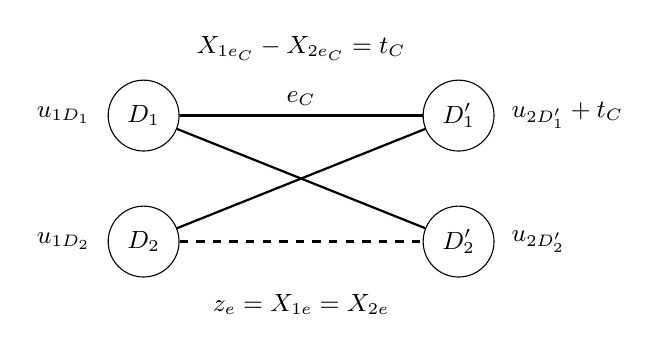
\begin{tikzpicture}[every node/.style={font=\small},
  vertex/.style={circle,draw,minimum size=9mm,inner sep=1pt}]
 \node[vertex] (a) at (0,1.6) {$D_1$};
 \node[vertex] (b) at (0,0) {$D_2$};
 \node[vertex] (c) at (4,1.6) {$D'_1$};
 \node[vertex] (d) at (4,0) {$D'_2$};
 \draw[thick] (a)--node[above] {$e_C$}(c);
 \draw[thick] (a)--(d);
 \draw[thick] (b)--(c);
 \draw[dashed,thick] (b)--(d);
 \node at (2,2.45) {$X_{1e_C}-X_{2e_C}=t_C$};
 \node at (2,-.8) {$z_e=X_{1e}=X_{2e}$};
 \node[anchor=east] at (-.55,1.6) {$u_{1D_1}$};
 \node[anchor=east] at (-.55,0) {$u_{1D_2}$};
 \node[anchor=west] at (4.55,1.6) {$u_{2D'_1}+t_C$};
 \node[anchor=west] at (4.55,0) {$u_{2D'_2}$};
\end{tikzpicture}
\caption{A schematic component with four edges. The solid edges form
the chosen tree; the dashed edge is a free coordinate. The displayed
right-hand margins are those for $X_1$. After solving the tree equations,
subtracting $t_C$ on $e_C$ gives the prescribed margins for $X_2$.
The construction applies to arbitrary bipartite multigraph components.}
\label{fig:tree-ports}
\end{figure}

Let $\mathcal F_G$ denote the nontree edges in a superblock $G$. In discrete sums
we take $z\in\{0,\ldots,R\}^{\mathcal F_G}$; for integration we use
$Q_G=[0,R+1]^{\mathcal F_G}$. These choices include every original base pair.
They also fix the measure: it is ordinary Lebesgue measure in $z$,
with a zero-dimensional integral equal to its integrand.

\subsection{Convex penalties and comparison with the count}

For each superblock $G$, let $A_{iG}$ be the union of blocks preceding
$G$ in the order for system $i$, with the reversed order for system 2.
Define the contracted ranks and their violation penalty by
\begin{align}
 r_{iG}(U)&=r_i(A_{iG}\cup U)-r_i(A_{iG})
       &&(U\subseteq G),\\
 V_G(u,z)&=\sum_{i=1}^2\max_{U\subseteq G}
                 \{X_i(u,z)(U)-r_{iG}(U)\},
 &\lambda&=N^{320}/W.\label{eq:block-penalty}
\end{align}
Each maximum includes the empty set, so $V_G$ is nonnegative and convex.
The hard conditions on ports are
\begin{equation}\label{eq:hard-port-conditions}
 u_i\in B(\bar r_i)\quad(i=1,2),\qquad
 \sum_{C\subseteq G}t_C=0\quad\hbox{for every }G.
\end{equation}

\begin{lemma}[What the penalties enforce]\label{lem:port-penalties}
An original base pair with a representative shift satisfies
\eqref{eq:hard-port-conditions} and $\sum_GV_G\le N^7S$.
Conversely, if~\eqref{eq:hard-port-conditions} holds, then
\[
 X_i(A)-r_i(A)\le\sum_G V_G\qquad(A\subseteq E, i=1,2).
\]
If in addition $\sum_GV_G\le T$, then $X_i\in B_i^+$ for both $i$,
where $B_i^+$ is defined in~\eqref{eq:expanded-bases}.
\end{lemma}

\begin{proof}
The representative shift has sum zero on each superblock, proving the
hard conditions. For an original pair, every forward superblock prefix $A$
satisfies $x_1(A)=x_2(A)$. Its two complementary rank slacks therefore
add to $s_*(A)\le N^4S$. The system-2 prefixes are complements of such
forward prefixes. In particular the slack at either prefix
$A_{iG}$ is at most $N^4S$. The inequality on $A_{iG}\cup U$ gives
\[
 x_i(U)-r_{iG}(U)\le r_i(A_{iG})-x_i(A_{iG}),
\]
so summing over the two systems and at most $n$ blocks proves the first
bound.

For the converse, fix $i$ and put $U_G=A\cap G$. Diminishing marginal
returns, applied successively in the order of system $i$, gives
\[
 \sum_G\bigl(r_i(A_{iG}\cup U_G)-r_i(A_{iG})\bigr)\le r_i(A).
\]
Indeed the prefix of the already selected pieces of $A$ is contained
in $A_{iG}$; its marginal increment from $U_G$ is at least the increment
from the full prefix. Summing the defining inequalities for $V_G$
proves the claim. The hard rank conditions enforce the correct total
and every inequality on a union of parts of $\mathcal D_i$. Any other
set cuts at least one part. Its rank bound in $B_i^+$ increases by
$T$ for every pair of coordinates in that part separated by the set,
and hence by at least $T$. This absorbs the remaining violation.
\end{proof}

Write $J=\sum_l\exp(-\sum_jl_j^2/M^2)$ for the normalizer of the
representative average of Lemma~\ref{lem:shift-average}. Consider
\begin{equation}\label{eq:discrete-port-sum}
 \mathcal A=\sum_{\substack{u\text{ in the integer port boxes}\\
                          \text{satisfying }\eqref{eq:hard-port-conditions}}}
 \ \sum_{z\in\{0,\ldots,R\}^{\bigcup_G\mathcal F_G}}
 \exp\left(-\lambda\sum_GV_G(u,z)
           -\sum_G\sum_{C\ne C_0(G)}t_C(u)^2/M^2\right).
\end{equation}
Under the hard block equality, the nonroot values $t_C$ are precisely
the independent representative star coordinates. Lemma~\ref{lem:tree-coordinates}
therefore identifies every summand with one representative-shift pair.
For a lower bound, retain original pairs with $|l_j|\le S/N^{25}$.
Their ports and free coordinates are in the chosen boxes, and their
additional penalty is at most
$\lambda N^7S=N^{327}S/W<N^{-20}$.
For an upper bound, the summands with $\sum_GV_G\le T$ form a subset
of the expanded representative average. The remaining summands have
total at most
\[
 e^K e^{-\lambda T}=\exp(K-N^{20}).
\]
The product bound associated with~\eqref{eq:scales} justifies $e^K$
here. Since $JZ\ge1$, this last bound is negligible also as a relative
error. Lemma~\ref{lem:shift-average} and
Proposition~\ref{prop:expansion} now give
\begin{equation}\label{eq:discrete-proxy-bound}
 \left|\log\frac{\mathcal A}{JZ}\right|\le40N^{-8}.
\end{equation}

Define the continuous block weights
\begin{equation}\label{eq:block-integral}
 I_G(u)=\int_{Q_G}\exp(-\lambda V_G(u,z))\dd z.
\end{equation}
They are positive. They are log concave by the theorem on marginals
of log-concave functions \cite{Prekopa1973}, applied to the integrand
times the indicator of its convex integration box. The tree coefficient
bound implies, globally in the joint variables $(u,z)$,
\begin{equation}\label{eq:port-lipschitz}
 |\lambda V_G(u,z)-\lambda V_G(u',z')|
 \le L_0\norm{(u,z)-(u',z')}_\infty,
 \qquad L_0=N^{330}/W.
\end{equation}
For example, at most $3n$ input variables, at most $n$ edge coordinates
per subset sum, and coefficients bounded by $10(n+1)$ give a Lipschitz
constant at most $100(n+1)^4\lambda<L_0$.
Integrating the corresponding pointwise ratio bounds proves the same
bound for $\log I_G$ in $u$. Define the hard integrated mass
\[
 \mathcal I_{\rm hard}
 =\sum_{\substack{u\text{ in the integer port boxes}\\
                    \text{satisfying }\eqref{eq:hard-port-conditions}}}
       \prod_G I_G(u)
       \exp\left(-\sum_G\sum_{C\ne C_0(G)}t_C(u)^2/M^2\right).
\]
Tiling $Q_G$ by unit cells anchored at
$\{0,\ldots,R\}^{\mathcal F_G}$ gives
\begin{equation}\label{eq:sum-integral-comparison}
 \left|\log\frac{\mathcal I_{\rm hard}}{\mathcal A}\right|\le2nL_0.
\end{equation}

\subsection{Smoothing and the paired count model}

We have obtained positive log-concave block integrals, but log concavity
alone does not imply either integer signature. We arrange a quantitative
version by smoothing on a scale on which the weights barely change,
then adding a smaller strictly concave quadratic.
Its strict Hessian margin will absorb the error between second
derivatives and the discrete differences in the signature test.
Set
\begin{equation}\label{eq:smoothing-scales}
 b_0=W/N^{400},\qquad \alpha=N^{-100}/W^2,\qquad H=N^{10}.
\end{equation}
In every port coordinate independently, let $\kappa_{b_0}$ be the law
of a sum of six uniform variables on $[-b_0/6,b_0/6]$. Convolve $I_G$
in its port variables with the product of these kernels, writing the
result as $\widetilde I_G$. The kernel and the integral are log concave,
so their convolution is log concave as well \cite{Prekopa1973}.
Its support displacement has sup norm at most $b_0$; hence
\begin{equation}\label{eq:smoothing-error}
 e^{-L_0b_0}I_G(u)\le\widetilde I_G(u)\le e^{L_0b_0}I_G(u).
\end{equation}
Define
\begin{equation}\label{eq:block-factor}
 F_G(u)=\widetilde I_G(u)\exp\left\{
 -\frac\alpha2\sum_{i,D\subseteq G}(u_{iD}-c(D))^2
 -\sum_{C\ne C_0(G)}\frac{t_C(u)^2}{M^2}
 -H\left|\sum_{C\subseteq G}t_C(u)\right|\right\}.
\end{equation}
For a rank $r$ on part indices, let
\[
 m_r(v)=\min_A\{r(A)+v(E_r\setminus A)\},\qquad
 \Phi_{r,H}(v)=\exp\{-H[v(E_r)+r(E_r)-2m_r(v)]\},
\]
where $E_r$ is its index set. This is the soft rank factor of
\eqref{eq:rank-soft-weight}. On nonnegative integral inputs its penalty
is nonnegative, is zero exactly on $B(r)$, and is at least $H$ otherwise.
The positive port weight is
\begin{equation}\label{eq:positive-port-weight}
 w(u)=\Phi_{\bar r_1,H}(u_1)\Phi_{\bar r_2,H}(u_2)\prod_GF_G(u).
\end{equation}
On the hard profiles the softened penalties vanish, and hence
\[
 \left|\log\frac{\sum_{u\text{ satisfying }\eqref{eq:hard-port-conditions}}
                                  w(u)}{\mathcal I_{\rm hard}}\right|
 \le nL_0b_0+\alpha n(N^{21}W)^2<N^{-50}.
\]
Every profile violating a hard condition has an integral nonzero
penalty and hence an extra factor at most $e^{-H}$. All other
exponential factors are at most one, and
$\widetilde I_G\le(R+1)^{|\mathcal F_G|}$. Thus
\[
 0\le\sum_u w(u)
      -\sum_{u\text{ satisfying }\eqref{eq:hard-port-conditions}}w(u)
      \le e^{K-H}.
\]
Combining these estimates with
\eqref{eq:discrete-proxy-bound} proves
\begin{equation}\label{eq:positive-proxy-bound}
 \left|\log\frac{\sum_u w(u)}{JZ}\right|\le100N^{-7}.
\end{equation}
The weighted port sum now approximates $JZ$. It remains to represent
this sum as a balanced mass of weights with both integer signatures.

To expose the disjoint factor groups needed for signatures, give each
positive-length port two count coordinates $(a_{iD},b_{iD})$, each of
capacity $d_{iD}$. The coordinate $a$ feeds a rank factor; $b$ feeds a
block factor. Their interpreted port values are
\begin{center}
\begin{tabular}{c@{\qquad}cc}
 & rank argument & block argument\\ \hline
 $i=1$ & $U_{1D}-a_{1D}$ & $L_{1D}+b_{1D}$\\
 $i=2$ & $L_{2D}+a_{2D}$ & $U_{2D}-b_{2D}$.
\end{tabular}
\end{center}
They agree exactly when $a_{iD}+b_{iD}=d_{iD}$. Length-zero ports are
fixed at their endpoint and omitted. All count coordinates are integers. Let
\begin{equation}\label{eq:paired-count-slice}
 p=\sum_{i,D}d_{iD},\qquad
 \mathcal S=\{(a,b):0\le a_{iD},b_{iD}\le d_{iD},\quad
                         \sum_{i,D}(a_{iD}+b_{iD})=p\}.
\end{equation}
Let $h$ on $\mathcal S$ be the product in
\eqref{eq:positive-port-weight}, using rank and block arguments from the
corresponding columns. The factors now use disjoint count coordinates.
The side-2 reflection makes every retained block coordinate enter its
component imbalance with coefficient $+1$:
\[
 t_C=\sum_{D\in C\cap\mathcal D_1}L_{1D}
       -\sum_{D\in C\cap\mathcal D_2}U_{2D}
       +\sum_{(i,D):D\in C}b_{iD},
\]
where omitted count coordinates are understood as zero. This common
orientation is needed for both imbalance factors in the signature test.

\subsection{The quantitative signature estimate}

\begin{lemma}[Derivatives after smoothing]\label{lem:smooth-derivatives}
In block count coordinates, $g=\log\widetilde I_G$ is $C^3$, is concave,
and satisfies, everywhere,
\begin{equation}\label{eq:smooth-derivative-bounds}
 |g''_{ij}|\le A_2=N^{800}/W^2,\qquad
 |g'''_{ijk}|\le A_3=N^{1250}/W^3.
\end{equation}
\end{lemma}

\begin{proof}
A uniform density on an interval of length $b_0/3$ has distributional
derivative of total variation $6/b_0$. Assigning at most three
derivatives to distinct uniform factors in each sixfold convolution
shows that every product-kernel derivative of total order $q\le3$
has total variation at most $6^qb_0^{-q}$. The remaining convolutions
give continuous derivatives through order three. Every positive-order
derivative has integral zero. Subtracting $I_G(u)$ inside its integral,
and using~\eqref{eq:port-lipschitz}, bounds each relative derivative of
$\widetilde I_G$ of order $q=1,2,3$ by
\[
 10^{11}L_0b_0^{1-q}.
\]
Here $e^{L_0b_0}-1\le2L_0b_0$, and
$\widetilde I_G(u)\ge e^{-L_0b_0}I_G(u)$.
The identities for derivatives of a logarithm give second derivatives
bounded by a constant times
$L_0/b_0+L_0^2$, and third derivatives bounded by a constant times
$L_0/b_0^2+L_0^2/b_0+L_0^3$; the constants from the preceding display
are absorbed by the powers in~\eqref{eq:smooth-derivative-bounds}.
For example $L_0/b_0=N^{730}/W^2$ and
$L_0/b_0^2=N^{1130}/W^3$. Reflection of side-2 coordinates only changes
derivative signs and conjugates the Hessian by a diagonal sign matrix.
Thus the bounds and concavity hold in the count convention as claimed.
\end{proof}

\begin{lemma}[Block signatures at every power]\label{lem:block-signatures}
For $0\le s\le1$, every block factor $F_G^s$ has both normalized
positive-semidefinite tests of~\eqref{eq:signature-normalization}:
$\one\one^{\mathsf T}-Q\succeq0$, for additions and removals.
\end{lemma}

\begin{proof}
Fix a display $b$ and a direction $\sigma\in\{-1,1\}$. Initially allow
repeated changes outside the box, where the defining positive formula
still makes sense. The normalized entry for a factor $F$ is
\[
 Q_{ij}=\frac{F(b)F(b+\sigma e_i+\sigma e_j)}
                  {F(b+\sigma e_i)F(b+\sigma e_j)}.
\]
Ignore the last, absolute-value term of~\eqref{eq:block-factor} for the
moment. The finite difference of the smoothed logarithm integrates its
Hessian along two unit segments. Comparing it with the Hessian at $b$
costs at most $4A_3$ in every entry, also when $i=j$. The auxiliary
quadratic has exact finite difference $-\alpha\mathbf1_{i=j}$. Thus
these two factors contribute
\[
 \exp(sD_{ij}),\qquad
 D_{ij}=g''_{ij}(b)-\alpha\mathbf1_{i=j}+e_{ij},\quad
 |e_{ij}|\le4A_3.
\]
The imbalance Gaussian contributes
$\gamma=\exp(-2s/M^2)$ when $i,j$ belong to the same nonroot component,
and contributes one otherwise. Let $B$ be the matrix of these latter
entries. Its complement is explicitly positive semidefinite:
\[
 \one\one^{\mathsf T}-B
   =(1-\gamma)\sum_{C\ne C_0(G)}\one_C\one_C^{\mathsf T}\succeq0,
\]
where $\one_C$ indicates the block coordinates incident to $C$.

We next compare $Q=B\circ\exp(sD)$, with entrywise operations, to its
linear approximation. The inequalities
$1-e^{-2s/M^2}\le2s/M^2$ and
$|e^x-1-x|\le2x^2$ for $|x|\le1$ give
\begin{equation}\label{eq:signature-error}
 \one\one^{\mathsf T}-Q
  =(\one\one^{\mathsf T}-B)-s g''(b)+s\alpha I+E,
 \qquad |E_{ij}|\le s\mathcal E,
\end{equation}
where one may take
\[
 \mathcal E=10A_3+100(A_2+\alpha+4A_3)^2
                     +10(A_2+\alpha)/M^2.
\]
More explicitly, the error entries in this identity are
\[
 E_{ij}=-sB_{ij}e_{ij}
       +s(1-B_{ij})(g''_{ij}(b)-\alpha\mathbf1_{i=j})
       -B_{ij}(e^{sD_{ij}}-1-sD_{ij}).
\]
All entries of $D$ have absolute value below one. The three terms
are bounded respectively by $4sA_3$,
$2s^2(A_2+\alpha)/M^2$, and
$2s^2(A_2+\alpha+4A_3)^2$. Since $s^2\le s$, they give the displayed
budget uniformly even for arbitrarily small positive $s$.
There are at most $2n$ block coordinates, so
$\norm{E}_{\rm op}\le2ns\mathcal E$. The scale choices give
\[
 \frac{2n\mathcal E}{\alpha}
 \le N^4\left(\frac{N^{1350}}W+
                 \frac{N^{1700}}{W^2}+N^{-3100}\right)<\frac12.
\]
Both the first term on the right of~\eqref{eq:signature-error} and
$-sg''(b)$ are positive semidefinite. The term $s\alpha I$ therefore
absorbs the error for every $s>0$. At $s=0$ the assertion is immediate.

Finally the total imbalance in a block is the sum of all its count
coordinates plus a constant. Put $v=\sum_{C\subseteq G}t_C(b)$.
Its absolute-value penalty multiplies
every normalized entry by the same number
\[
 \beta=\exp\{-sH(|v+2\sigma|-2|v+\sigma|+|v|)\}\in(0,1].
\]
Since
$\one\one^{\mathsf T}-\beta Q
=(1-\beta)\one\one^{\mathsf T}
 +\beta(\one\one^{\mathsf T}-Q)$,
the test persists. Discard unavailable single changes and set the
diagonal to zero for invalid repeated changes. These operations take
principal matrices and add a nonnegative diagonal to their complements,
so they also preserve the test.
\end{proof}

\begin{proposition}[The positive port model]\label{prop:port-model}
For every nonempty input after the deterministic feasibility test,
the preceding construction gives at most $2n$ paired ports of lengths
$d_{iD}\le N^{21}W$, with $p=\sum d_{iD}$ polynomial in $N$, and a
strictly positive weight $h$ on the entire slice~\eqref{eq:paired-count-slice}.
For every real $s\in[0,1]$, $h^s$ has both integer signatures of
Definition~\ref{def:integer-signatures}. Its balanced mass
\[
 \mathcal Z_{\rm port}
   =\sum_{\substack{(a,b)\in\mathcal S\\
                    a_{iD}+b_{iD}=d_{iD}\ \forall(i,D)}}h(a,b)
\]
satisfies
$|\log(\mathcal Z_{\rm port}/(JZ))|\le100N^{-7}$.
These statements include $p=0$, when there is a single profile.
\end{proposition}

\begin{proof}
The balanced profiles are in bijection with the original integer port
settings, and their weights are $w(u)$, so
\eqref{eq:positive-proxy-bound} proves the comparison. Positivity is
explicit in the definitions. Lemma~\ref{lem:rank-signatures} applies
to the rank factors, including the simultaneous reflection on side 1.
Lemma~\ref{lem:block-signatures} applies to every block factor. The
coordinate groups of all these factors are disjoint; hence the full
normalized complement is the direct sum of their normalized
complements. The signature criterion in
Section~\ref{sec:signatures} proves the result.
\end{proof}

\section{Evaluating the weights with bounded rational computation}
\label{sec:evaluation}

The block integrals in Section~\ref{sec:ports} are definitions of weights,
not oracles supplied with the input. We now construct their evaluators.
The central step expresses a close approximation to an exponential
integral as the volume of a rational polytope. We check its separation
oracle, encoding lengths, and inner and outer geometric guarantees.
These checks also explain why a free-coordinate interval of length
$R+1$ causes only polynomial dependence on $\log(R+1)$.

\subsection{Magnitude bounds before numerical approximation}

\begin{lemma}[Integral and point-weight bounds]\label{lem:weight-bounds}
For every block and every port argument in its box,
\begin{equation}\label{eq:integral-bounds}
 e^{-N^{50000}}\le\widetilde I_G(u)\le e^K.
\end{equation}
For the weight $h$ on the full paired slice of
Proposition~\ref{prop:port-model},
\begin{equation}\label{eq:weight-log-bound}
 |\log h(a,b)|\le N^{60000}.
\end{equation}
All rational coefficients needed to define or evaluate its factors
have polynomial encoding length in the input and in the query.
\end{lemma}

\begin{proof}
The integral's upper bound is its free-box volume,
$(R+1)^{|\mathcal F_G|}\le e^K$, since smoothing uses probability kernels.
For the lower bound put $u^c_{iD}=c(D)$ and $z^c_e=c_e$ on free edges.
The tree solve gives $X_1=X_2=c$, so the prefix-slack argument of
Lemma~\ref{lem:port-penalties} gives
$V_G(u^c,z^c)\le2N^4S$. For each free coordinate choose
$z^*_e=\max\{c_e,1/4\}$. It lies in $[0,R+1]$ with at least $1/4$
clearance from its boundary and differs from $c_e$ by at most $1/4$.
On the cube of sup radius $1/8$ about $z^*$, and for every smoothing
displacement, the port and free-coordinate displacements from
$(u^c,z^c)$ are at most $N^{21}W+b_0+1$. Therefore
\begin{equation}\label{eq:near-center-penalty}
 \lambda V_G(u-v,z)
 \le2\lambda N^4S+L_0(N^{21}W+b_0+1)<N^{5000}.
\end{equation}
Integrating over this cube and over the whole probability kernel gives
$\widetilde I_G(u)\ge4^{-|\mathcal F_G|}e^{-N^{5000}}
\ge e^{-N^{50000}}$. This proof includes $\mathcal F_G=\varnothing$.

For the rank factors, choose any common integral base $x^*$, which
exists by the feasibility and integrality results of Section~\ref{sec:polyhedra}.
Its projected totals $v^*_i$ satisfy the rank constraint and are within
$N^{10}W$ of the center totals by~\eqref{eq:part-total-range}.
For any nonnegative vector $v$ on a rank index set, its rank penalty is
\[
 v(E_r)+r(E_r)-2m_r(v)
  =\max_{A\subseteq E_r}
       \{v(A)-v(E_r\setminus A)+r(E_r)-2r(A)\}.
\]
Every affine function on the right has coordinate slopes $\pm1$.
Thus this penalty is 1-Lipschitz in the $1$-norm. It vanishes at $v_i^*$,
so throughout a port box it is at most $N^{23}W$, independently of the
numerical value of $R$. Multiplication by $H$ still gives a fixed power
of $N$. For each component, $t_C$ vanishes at the center and has
absolute value at most $N^{23}W$ throughout the boxes. Consequently
all Gaussian and absolute-value exponents in~\eqref{eq:block-factor}
have absolute value bounded by fixed powers below $N^{40000}$; the
auxiliary quadratic is smaller than one. Summing these bounds and
\eqref{eq:integral-bounds} over at most $n$ blocks proves
\eqref{eq:weight-log-bound}.

The center, endpoints, scales, and tree coefficients have polynomial
encoding length. Ranks of unions and contracted ranks require ordinary
rank queries. For the minima defining $m_r$ and the maxima defining
$V_G$, rational modular terms are handled by clearing their common
denominator and applying Proposition~\ref{prop:oracle-tools}. The binary
length of that denominator is at most the sum of the individual
denominator lengths. Thus the size parameter is polynomial in bits;
no bound on its numerical value is needed.
\end{proof}

\subsection{A rational volume problem}

We use the following form of the classical randomized volume theorem
\cite{DFK1991,DyerFrieze1991}. In dimension $d$, a full-dimensional
rational polytope supplied by strong separation, a polynomial bound
on each inequality's encoding length, and rational inner and outer
ball guarantees admits a relative volume approximation with success
probability at least $3/4$. Its oracle and bit complexity is polynomial
in $d$, these encoding lengths, and the reciprocal error. The radii
enter through their binary lengths. We use the finite-precision volume
algorithm in the rational oracle model of
\cite[Section~2]{DyerFrieze1991}. Its polynomial random-bit bound is
recorded in \cite[Section~6]{DyerFrieze1991}; finite-grid sampling within
cubes and its error analysis appear in
\cite[algorithm Step~2 and its finite-grid error analysis]{DFK1991}.
Finite uniform integer choices can be generated from unbiased bits by
rejection using fewer than two expected trials. The resulting expected
polynomial bound includes bit operations, rational arithmetic, and
oracle calls; we cap and amplify this procedure below. Strong separation
supplies the weak membership required in the volume theorem.

We first round each volume input by a rational change of coordinates.
Apply Lemma~\ref{lem:center} to the full-dimensional
polytope and send its returned simplex vertices to $0,e_1,\ldots,e_d$.
The image contains the standard simplex and lies in $[-2,2]^d$,
because its nonconstant barycentric coordinates have absolute value
at most two. The standard simplex contains a Euclidean ball about
its barycenter of radius at least $(d+1)^{-2}$. Translating that
barycenter to zero and scaling by $(d+1)^2$ therefore give an inner
unit ball and an outer ball of polynomial radius. The affine map,
its determinant, and the inverse images of rational separation queries
have polynomial encoding length. Correcting the returned volume by
the determinant is exact rational arithmetic. The required optimization
uses the rational separation theorem \cite{GLS1988}, through
Proposition~\ref{prop:oracle-tools}. This supplies a rounded input
even when the original geometric aspect ratio is numerically large.

Fix a block and a rational port vector $u$ in its box. Let $m$ be the
number of its port arguments, including fixed length-zero ports, and
$f=|\mathcal F_G|$ its number of free variables. Length-zero ports are
omitted only from the count slice; they remain arguments of the smoothing
convolution.
Replace its $6m$ uniform variables by $q_{ja}\in[0,1]$, putting
\[
 v_j(q)=\frac{b_0}{3}\sum_{a=1}^6(q_{ja}-1/2),\qquad
 \mathcal B=[0,R+1]^f\times[0,1]^{6m},\qquad
 D(z,q)=\lambda V_G(u-v(q),z).
\]
The normalized uniform density has been absorbed by this unit-interval
parametrization, so there is no further Jacobian factor:
\begin{equation}\label{eq:exponential-box-integral}
 \widetilde I_G(u)=\int_{\mathcal B}e^{-D(x)}\dd x,
 \qquad x=(z,q).
\end{equation}
Here $D$ is nonnegative, convex, and piecewise affine. Its value and an
attaining affine piece can be computed exactly at rational points:
submodular minimization returns a maximizing subset for each of the
two maxima in $V_G$, and their sum is such a piece.

For $0<\rho<1$, define
\begin{equation}\label{eq:volume-lift-scales}
 E_0=N^{51000}+\lceil\log_2(100/\rho)\rceil,
 \qquad d_0=\lceil1000E_0^2/\rho\rceil.
\end{equation}
The ceiling of the logarithm can be found by integer comparisons of
powers of two, without numerical logarithms. Consider the polytope
\begin{equation}\label{eq:volume-lift}
 \mathcal Q=\{(x,y):x\in\mathcal B,\ y\in\R_{\ge0}^{d_0},\quad
                   D(x)+d_0y_a\le d_0\ (1\le a\le d_0)\}.
\end{equation}
Each inequality involving $D$ means all the affine-piece inequalities
in its finite maximum representation. This makes $\mathcal Q$ a
convex rational polytope, although its inequalities are not enumerated.
Integrating over its $y$-fiber gives the exact identity
\begin{equation}\label{eq:fiber-volume}
 \vol(\mathcal Q)=\int_{\mathcal B}(1-D(x)/d_0)_+^{d_0}\dd x.
\end{equation}

\begin{lemma}[Accuracy and guarantees for the volume lift]
\label{lem:volume-lift}
The polytope~\eqref{eq:volume-lift} has dimension $f+6m+d_0$, a
polynomial facet-encoding bound, and an exact polynomial-time strong
separation oracle. It contains a known rational ball of radius $1/32$
and has an outer ball of polynomial encoding length. Furthermore,
\begin{equation}\label{eq:volume-lift-accuracy}
 (1-\rho/10)\widetilde I_G(u)
       \le\vol(\mathcal Q)\le\widetilde I_G(u).
\end{equation}
All polynomial bounds are in the original input length, the encoding
lengths of $u$ and $\rho$, $N$, and $\rho^{-1}$, with absolute fixed exponents.
\end{lemma}

\begin{proof}
The pointwise upper inequality follows from $1-t\le e^{-t}$. For
$0\le D\le E_0$, expansion of $-\log(1-t)$, or integration of its
derivative, gives
\[
 0\le-d_0\log(1-D/d_0)-D
 \le\frac{D^2}{2d_0(1-D/d_0)}<\rho/100.
\]
The part of~\eqref{eq:exponential-box-integral} where $D>E_0$ has
integral at most $e^{K-E_0}$. Dividing by the lower bound in
\eqref{eq:integral-bounds} makes its relative contribution at most
\[
 \exp(K+N^{50000}-E_0)<\rho/100.
\]
These two errors prove~\eqref{eq:volume-lift-accuracy}.

For separation, first test the box inequalities and $y\ge0$. Compute
$D(x)$ and choose an index $a$ with largest $y_a$. If
$D(x)+d_0y_a>d_0$, the attaining affine piece of $D$ gives a rational
hyperplane separating the point from $\mathcal Q$. Otherwise all
inequalities hold. The coefficient bounds follow from the integral
tree map, the rank-answer bit bound, the rational scales, and the
input port encodings. At a rational query, clearing denominators for
the two submodular minimizations takes polynomial bit work as in
Lemma~\ref{lem:weight-bounds}. Each inequality, rather than the number
of possible subsets, is the encoding parameter.

For the inner ball choose
\[
 x^*=(z^*,q^*),\qquad z^*_e=\max\{c_e,1/4\},\qquad
 q^*_{ja}=1/2,\qquad y^*_a=1/4.
\]
All box coordinates have clearance at least $1/4$. A Euclidean
perturbation of radius $1/32$ changes each free coordinate by at most
$1/32$ and each $v_j$ by at most $2b_0/32$. By
\eqref{eq:port-lipschitz} its change in $D$ is at most
$L_0\max\{1,2b_0\}/32<1$. The near-center estimate
\eqref{eq:near-center-penalty} therefore gives $D<N^{5000}+1<d_0/2$
throughout this ball. Also $0<y_a\le9/32$, so
$D+d_0y_a<25d_0/32<d_0$. This proves the inner guarantee, including
$f=0$. Every point of $\mathcal Q$ has $x\in\mathcal B$ and
$0\le y_a\le1$. If $d=f+6m+d_0$, the ball centered at the origin
with rational radius $d(R+2)$ is therefore an outer ball. Its binary
encoding length is polynomial.

Finally, the numerical value of $d_0$ is polynomial in $N$ and
$\rho^{-1}$: the exponents in~\eqref{eq:volume-lift-scales} are fixed.
Thus even its explicitly added coordinates can be written and
processed within one fixed polynomial bound. The original capacity
appears only in the box endpoint $R+1$ and the encoding lengths just
verified.
\end{proof}

\subsection{Positive rational outputs and deterministic caps}

\begin{proposition}[A bounded weight evaluator]\label{prop:weight-evaluator}
Given a profile in the entire slice $\mathcal S$, rational
$0<\rho,\beta<1$, and a rational power $s\in[0,1]$ with denominator
$q_s$, there is an evaluator using fresh random bits and returning a strictly positive rational
$\widehat h_s$ such that
\[
 \PP\bigl[(1-\rho)h^s\le\widehat h_s\le(1+\rho)h^s\bigr]
       \ge1-\beta.
\]
Its output length, number of rank queries, and other bit operations
are bounded on every execution by fixed polynomials in $N$, the
input encoding lengths, $\rho^{-1}$, $\log(\beta^{-1})$, and $q_s$.
In particular an equally spaced schedule with a polynomial number of
phases has polynomially bounded denominators. Moreover $J$ admits
a deterministic positive rational approximation $\widehat J$ with
$|\log(\widehat J/J)|\le N^{-7}$ in polynomial work.
\end{proposition}

\begin{proof}
First evaluate a single smoothed block integral. Round $\mathcal Q$
by the rational affine construction above, apply the volume theorem
with relative error $\rho/10$, and restore the exact determinant factor.
Use the same parameter $\rho$ in~\eqref{eq:volume-lift-scales}. By
Lemma~\ref{lem:volume-lift}, its successful output is a relative
$\rho/2$ approximation to $\widetilde I_G$.

For completeness, all resource bounds here are bounds on actual
finite-bit executions. Let $B$ be a furnished polynomial upper bound
on the expected combined number of bit operations and oracle calls
of one volume run, including the cost of its separation queries.
If the chosen version already has a deterministic bound, use that
bound instead. Interrupt the run after $16B$ operations; Markov's
inequality increases the failure probability by at most $1/16$.
The resulting success probability is at least $11/16$. On interruption,
a declared failure (including a zero denominator), or an invalid or
nonpositive output, substitute a fixed positive rational. Repeat independently
$O(1+\log\beta^{-1})$ times and take the median. The binomial tail
bound gives failure probability at most $\beta$. Cap construction,
query lengths, arithmetic, and random-bit generation are all included.
Clip each output to
\[
 [2^{-2N^{50000}},\ 2^{2N^{50000}}].
\]
This interval has polynomial-bit endpoints and strictly contains all
successful relative approximations from~\eqref{eq:integral-bounds}.
Clipping therefore retains the success guarantee and ensures bounded
positive outputs even on failed or interrupted runs.

Evaluate all rank penalties and the other rational exponents exactly,
and allocate relative error $\rho/(100(n+1))$ and failure allowance
$\beta/(n+1)$ to each of the at most $n$ block integrals. Evaluate the
remaining exponentials and all rational arithmetic to another
$\rho/(100(n+1))$ relative error per factor. The log bounds in
Lemma~\ref{lem:weight-bounds} ensure that these relative accuracies
require only polynomial absolute precision. One elementary
implementation uses the exponential Taylor series and factorial tail
bounds: an exponent of magnitude at most $D_*$ and absolute precision
$2^{-k}$ require polynomially many terms and bits in $D_*+k+1$.
Negative exponents can be evaluated by inversion of a positive
exponential approximation. Here $D_*$ is a fixed polynomial in $N$,
not in $R$.

Multiplying the factors gives a positive relative approximation to
$h$. Before taking any power, clip this product to
$[2^{-3N^{60000}},2^{3N^{60000}}]$. This interval contains $h$ by
\eqref{eq:weight-log-bound}, so clipping cannot increase its relative
error; it also gives valid bisection bounds even after failed block
evaluations. On the simultaneous success event the sum of the factor
logarithmic errors is below $\rho/10$, after reducing the indicated
constants if necessary. To obtain $h^s$ for $s=a_s/q_s$, apply bisection to the
$q_s$th root and integer powering to $a_s$, with positive rational
endpoints whose binary exponents are bounded by
$3N^{60000}$. Each comparison is an integer-power comparison, and
$a_s\le q_s$; the number of bisections, lengths of operands, and
bit work are polynomial in $q_s$, $N$, and $\log\rho^{-1}$.
Taking a power in $[0,1]$ cannot increase the preceding logarithmic
error. Approximate the root to logarithmic error at most
$\rho/[100(q_s+1)]$ before taking the $a_s$th power; the resulting
additional logarithmic error is at most $\rho/100$. This proves the
required relative bound. For $s=0$ return one exactly.
All steps have prescribed finite bounds; clipping the final output
to $[2^{-3N^{60000}},2^{3N^{60000}}]$ gives the same positivity and
encoding guarantee on every failure event. This proves the asserted
evaluator without conditioning any future computation on its success.

To approximate $J$, let $k$ be the number of nonroot components, so
\[
 J=\left(\sum_{j\in\Z}e^{-j^2/M^2}\right)^k,
 \qquad 0\le k\le n.
\]
For $k=0$ return one. Otherwise truncate at the integer
$B_J=MN^{10}$, a polynomial in $N$. The omitted two-sided tail is at
most
\[
 2\int_{B_J}^{\infty}e^{-x^2/M^2}\dd x
 \le\frac{M^2}{B_J}e^{-B_J^2/M^2}
 =MN^{-10}e^{-N^{20}}.
\]
The sum is at least one. Approximate each of its $2B_J+1$ retained
terms to absolute error at most
$N^{-7}/[100(n+1)(2B_J+1)]$, keeping the term at zero exactly one
and the remaining terms nonnegative. The elementary exponential
procedure above is bounded since each exponent has magnitude at most
$N^{20}$. Adding the terms and raising to the integer power $k$
gives a positive rational result whose logarithmic error is below
$N^{-7}$. No random choices or numerical grid of length $R$ occurs.
\end{proof}

\section{Counting the balanced port profiles}
\label{sec:counting}

The port model of Proposition~\ref{prop:port-model} and the evaluator
of Proposition~\ref{prop:weight-evaluator} give a sum of positive weights
on polynomially short ranges whose individual terms we can approximate.
We now approximate the entire sum.
The factorial encoding below is essential: its transversals have exactly
the mass of the unlabelled port profiles.  The two resulting binary weights
allow us to use the transport and trace estimates of the common-base
framework, in the two-weight form proved in~\cite{CB}.

Write $\mathcal P$ for the positive-length ports and $d_v$ for the length
of port $v\in\mathcal P$.  Thus $p=\sum_v d_v$, and the weight $h$ of
Proposition~\ref{prop:port-model} is positive on the entire slice
\[
 \mathcal B_p=\left\{(a,b):0\leq a_v,b_v\leq d_v,
                  \quad\sum_v(a_v+b_v)=p\right\}.
\]
All count coordinates in this section are integers.  The quantity to be
estimated is
\begin{equation}
 \mathcal Z_{\rm port}
   =\sum_{\substack{(a,b)\in\mathcal B_p\\a_v+b_v=d_v\ (v\in\mathcal P)}}
           h(a,b),
 \qquad
 \left|\log\frac{\mathcal Z_{\rm port}}{JZ}\right|
        \leq100N^{-7}.
 \label{eq:counting-target}
\end{equation}
Length-zero ports have already been fixed in $h$.  If $p=0$, the sum has
one term; we evaluate it directly at the end of the proof.  Until then
assume $p\geq1$.

\subsection{Two factorial weights and their signatures}

For every port $v$, introduce $d_v$ labelled pairs, each containing an
$a$-element and a $b$-element.  Let $\mathcal E$ be this ground set of
$2p$ elements and number its pairs $1,\ldots,p$.  For every $p$-subset
$S\subseteq\mathcal E$, its counts $(a(S),b(S))$ belong to
$\mathcal B_p$.  Given a positive count weight $k$ on this slice, define
\begin{equation}
 f(S)=k(a,b)\prod_{v\in\mathcal P}\frac{a_v!b_v!}{d_v!},
 \qquad
 \widetilde f(S)=k(a,b)
       \prod_{v\in\mathcal P}\frac{(d_v-a_v)!(d_v-b_v)!}{d_v!}.
 \label{eq:counting-lifts}
\end{equation}
Both weights are defined and positive on \emph{every} $p$-subset, including
subsets with several empty or full pairs.

Let $\mathcal A$ consist of the transversals, which select exactly one
element from each pair.  For distinct labels $i,l$, let $\mathcal A_{il}$
consist of the subsets with pair $i$ empty, pair $l$ full, and every
other pair singly occupied.  On a transversal the two factors in
\eqref{eq:counting-lifts} coincide and equal
$\prod_v\binom{d_v}{a_v}^{-1}$.  Exactly
$\prod_v\binom{d_v}{a_v}$ transversals realize any balanced profile.
Consequently
\begin{equation}
 C:=\sum_{S\in\mathcal A}f(S)
   =\sum_{S\in\mathcal A}\widetilde f(S)
   =\sum_{a+b=d}k(a,b).
 \label{eq:counting-multiplicity}
\end{equation}
This identity concerns transversals, rather than all subsets with the
same coordinate counts.

For a positive weight on all $r$-subsets of a finite set, the
\emph{addition property} means that, after any $r-2$ elements have
been fixed included, the matrix of weights obtained by adding two
distinct further elements, with zero diagonal, has at most one positive
eigenvalue.  It is vacuous for $r<2$.  The \emph{omission property} is
the addition property of the complement-set weight.

\begin{lemma}
\label{lem:counting-lifts}
If $k$ has both integer signatures of Definition~\ref{def:integer-signatures},
then $f$ has the omission property and $\widetilde f$ has the addition
property.  Both properties persist under fixing included or excluded
elements and summing disjoint labelled pairs at occupancy one, on each
resulting full valid-degree domain.  Moreover, with $q=(p+1)^2$,
\begin{equation}
 q^{-1}f(S)\leq\widetilde f(S)\leq qf(S)
 \quad\left(S\in\mathcal A\cup\bigcup_{i\ne l}\mathcal A_{il}\right).
 \label{eq:counting-comparison}
\end{equation}
\end{lemma}

\begin{proof}
We give the factorial cancellation in
\cite[Lemma~4.2, ``Signatures of the two lifts'']{CB}, since it also
explains the roles of the two weights.  In an omission test for $f$,
the display has $p+2$ elements.  Group these by count coordinate and let
$n_u$ be the number in group $u$.  On the subspace of vectors constant
within each group, the ordered-copy multiplicities $n_un_w$ for $u\ne w$
and $n_u(n_u-1)$ for $u=w$ cancel the factorial reductions from removing
two elements.  The quadratic form becomes
\[
 \frac{\prod_u n_u!}{\prod_v d_v!}
       \sum_{u,w}k(n-e_u-e_w)t_ut_w,
\]
where invalid removals contribute zero.  Its positive index is at most
one by the integer removal signature.  Vectors summing to zero within
each group have nonpositive quadratic form and are orthogonal for this
form to the group-constant subspace: within a group the matrix has
constant nonnegative off-diagonal entries and zero diagonal.  This
proves the omission assertion.  For $\widetilde f$, group the elements
available after fixing $p-2$ inclusions.  The remaining-capacity
factorials cancel the same multiplicities, leaving a positive multiple
of the integer addition matrix.  This proves the addition assertion.
The closure assertions are precisely
\cite[Lemma~4.1, ``Binary contractions'']{CB}; their hypothesis of
positivity on the full domain has been checked here.

For the comparison, if the empty and full pair are in the same port,
all ports remain balanced and the ratio is one.  Otherwise the port
containing the hole has $a+b=d-1$, and contributes $(a+1)(b+1)$
to $\widetilde f/f$.  The port containing the full pair has
$a+b=d+1$ and contributes $1/(ab)$.  Both positive integer products
lie between $1$ and $(p+1)^2$.  Their quotient proves
\eqref{eq:counting-comparison}.
\end{proof}

\subsection{The transport input and the chain it controls}

We state the precise consequence of the companion transport argument
that will be used.  This isolates the long transport proof from the
algorithm and makes its hypotheses available for verification.
Fix $f,\widetilde f$ as above and put
$c_{il}=\sum_{S\in\mathcal A_{il}}f(S)$.  These numbers are positive.
For positive multipliers $w_{il}$ define, on
$\mathcal X=\mathcal A\cup\bigcup_{i\ne l}\mathcal A_{il}$,
\[
 \lambda(S)=
 \begin{cases}f(S),&S\in\mathcal A,\\
               w_{il}f(S),&S\in\mathcal A_{il},\end{cases}
 \quad
 \Lambda=\sum_{S\in\mathcal X}\lambda(S),
 \quad \pi(S)=\lambda(S)/\Lambda,
 \quad \mu(S)=f(S)/C\quad(S\in\mathcal A).
\]
Call the multipliers \emph{good} when
\begin{equation}
 \frac{C}{4c_{il}}\leq w_{il}\leq\frac{4C}{c_{il}}
 \qquad(i\ne l).
 \label{eq:counting-good}
\end{equation}
In this case
\begin{equation}
 \Lambda\leq5p^2C,\qquad
 \pi(\mathcal A)\geq(5p^2)^{-1},\qquad
 \pi(\mathcal A_{il})\geq(20p^2)^{-1}.
 \label{eq:counting-type-mass}
\end{equation}

The chain holds with probability $1/2$.  Otherwise it chooses independently
a uniform element of $S$ and a uniform element of $\mathcal E\setminus S$,
and proposes their exchange.  A proposal outside $\mathcal X$ is rejected;
a proposal $S'\in\mathcal X$ is accepted with probability
$\min(1,\lambda(S')/\lambda(S))$.  Write $P$ for this kernel.  A defect
state can reach a transversal by moving an element of its full pair to
its empty pair, and transversals are connected by flips within pairs.
Thus positivity makes $P$ irreducible.  It is lazy and reversible, with
Dirichlet form
\begin{equation}
 \mathcal E_P(g)=\langle g,(I-P)g\rangle_\pi
   =\frac{\mathfrak D(g)}{2p^2\Lambda},\qquad
 \mathfrak D(g)=\sum_{\{S,S'\}}
      \min(\lambda(S),\lambda(S'))(g(S)-g(S'))^2,
 \label{eq:counting-energy}
\end{equation}
where the sum is over unordered exchange edges.
Let $\mathcal Qg$ agree with $g$ at each transversal and replace its
values on each defect class by their conditional $\pi$-mean.

\begin{proposition}[Companion transport and simulation input]
\label{prop:counting-transport}
Suppose $f$ is positive on all $p$-subsets and has the omission property,
$\widetilde f$ is positive on that domain and has the addition property,
the weights agree on $\mathcal A$, and
\eqref{eq:counting-comparison} holds with $q\geq1$.
For good multipliers put
\begin{equation}
 C_{\rm p}=p(1+8pq^2),\qquad
 C_{\rm d}=8+32pq^3,\qquad
 K_{\rm obs}=10p^4(9C_{\rm p}+2C_{\rm d}).
 \label{eq:counting-constants}
\end{equation}
Then for every real function $g$ on $\mathcal X$,
\begin{equation}
 C\operatorname{Var}_\mu(g)\leq C_{\rm p}\mathfrak D(g),\qquad
 \operatorname{Var}_\pi(\mathcal Qg)
 \leq(9C_{\rm p}+2C_{\rm d})\frac{\mathfrak D(g)}C
 \leq K_{\rm obs}\mathcal E_P(g).
 \label{eq:counting-variance}
\end{equation}
If $\mathcal QG=G$ and an initial law satisfies $\nu\leq D\pi$
pointwise, then $m\geq1$ consecutive observations satisfy
\begin{equation}
 \mathbb E_\nu\left[
  \left(m^{-1}\sum_{t=0}^{m-1}G(S_t)-\mathbb E_\pi G\right)^2\right]
 \leq\frac{2D K_{\rm obs}}m\operatorname{Var}_\pi(G).
 \label{eq:counting-time-average}
\end{equation}
The trace on $\mathcal A$, counting every strictly positive return as
one step, is lazy and reversible with stationary law $\mu$ and inverse
spectral gap at most $2p^2C_{\rm p}\leq K_{\rm obs}$.  In particular,
\begin{equation}
 \left|\frac{P_{\rm tr}^t(x,y)}{\mu(y)}-1\right|
 \leq\mu_{\min}^{-1}\exp(-t/K_{\rm obs}).
 \label{eq:counting-trace-mixing}
\end{equation}
If a trace starts from $\nu\leq D\mu$, the expected cost of $t$ trace
steps in underlying transitions is at most $tD/\pi(\mathcal A)$;
at each deterministic trace index its law is still at most $D\mu$.
\end{proposition}

\begin{proof}[Source and applicability]
These are \cite[Propositions~5.2 and~5.4 and Lemmas~5.5--5.6]{CB},
with $q$ left as the comparison parameter in their proofs.  Their
structural inputs are Lemma~5.1 (one-hole transport) and Lemma~4.4
(pair inequalities for defect masses).  We spell out why the stated
hypotheses are the complete interface.  For a partial transversal
assignment $\sigma$, let $z_\sigma$ be its transversal mass and let
$\widetilde c_{il}^{\sigma}$ be the mass of its extensions in
$\mathcal A_{il}$ under $\widetilde f$.  Binary contraction, including
the full-index cubic contraction clause of \cite[Lemma~4.1]{CB},
and the addition property give
\[
 4\widetilde c_{il}^{\sigma}\widetilde c_{li}^{\sigma}\leq z_\sigma^2,
 \qquad
 \widetilde c_{il}^{\sigma}\widetilde c_{lk}^{\sigma}
       \leq z_\sigma\widetilde c_{ik}^{\sigma}
 \quad(i,l,k\text{ distinct and unassigned}).
\]
Agreement on transversals identifies $z_\sigma$ for the two weights.
The omission property supplies one-hole transport for $f$, including
its auxiliary displays outside $\mathcal X$; this is why positivity
and the signature were required on all $p$-subsets.
Comparison on actual defect classes costs $q^2$ in the transversal
variance bound and $q^3$ in the defect-mean bound, giving exactly
$C_{\rm p},C_{\rm d}$ above.  The remaining observable and trace
arguments use only these inequalities, reversibility, and laziness.
They impose no condition on the origin of the count weight.
This is the two-lift version of the transport, observable-Poincare,
and trace-restart framework of~\cite[Sections~4--6]{Parent}.
\end{proof}

\subsection{Power annealing and exact initialization}

Lemma~\ref{lem:weight-bounds} gives $|\log h|\leq N^{60000}$, and
Proposition~\ref{prop:port-model} gives both integer signatures for
$h^s$ at every $0\leq s\leq1$.
Choose
\begin{equation}
 U=N^{61000},\qquad H_o=10U,\qquad
 k_j=(2^{-U}h)^{j/H_o}\quad(0\leq j\leq H_o),
 \qquad K_o=10(p+U+1).
 \label{eq:counting-schedule}
\end{equation}
Apply \eqref{eq:counting-lifts} to $k_j$, obtaining $f_j,\widetilde f_j$,
and denote their transversal and defect masses by $C_j,c_{il}(j)$.
Lemma~\ref{lem:counting-lifts} verifies every structural hypothesis of
Proposition~\ref{prop:counting-transport} at every phase, with
$q=(p+1)^2$.  In particular
\begin{equation}
 C_{H_o}=2^{-U}\mathcal Z_{\rm port}.
 \label{eq:counting-final-scale}
\end{equation}

\begin{lemma}[Initialization and adjacent phases]
\label{lem:counting-initialization}
For every $p$-subset and $0\leq j<H_o$,
\begin{equation}
 \frac12\leq\frac{f_{j+1}(S)}{f_j(S)}\leq1.
 \label{eq:counting-adjacent}
\end{equation}
Thus $C_j/c_{il}(j)$ changes by a factor in $[1/2,2]$ between
consecutive phases, and $\mu_j=f_j/C_j$ on $\mathcal A$ satisfies
$\mu_j\leq2\mu_{j+1}$.  Moreover
\begin{equation}
 \min_{S\in\mathcal A}\mu_j(S)
       \geq2^{-(H_o+p+K_o)}.
 \label{eq:counting-minimum}
\end{equation}
The initial masses are exact rational numbers computable in polynomial
bit time, and $\mu_0$ can be sampled by independent uniform port counts
followed by uniform subsets of the pairs realizing those counts.
\end{lemma}

\begin{proof}
The logarithm of $2^{-U}h$ lies between
$-U\log2-N^{60000}$ and $-U\log2+N^{60000}<0$.
Dividing by $H_o=10U$ proves \eqref{eq:counting-adjacent}.
Summing that bound within each type proves the multiplier comparison
and domination.  On a transversal the factorial factor is at least
$2^{-p}$, while $k_j\geq2^{-H_o}$.  Also
\[
 C_j\leq C_0=\prod_{v\in\mathcal P}(d_v+1)\leq2^p\leq2^{K_o},
\]
which proves \eqref{eq:counting-minimum}.

Here are explicit formulas for the initializer, as in
\cite[Lemma~7.1, ``Exact initialization'']{CB}.  Fix $i\ne l$.
For each port put
\[
 u_v=\mathbf1_{\{i\text{ lies in }v\}},\quad
 v_v=\mathbf1_{\{l\text{ lies in }v\}},\quad
 m_v=d_v-u_v-v_v.
\]
There are $m_v$ singly occupied pairs left in this port, so
\begin{equation}
 c_{il}(0)=\prod_{v\in\mathcal P}
 \left[\frac1{d_v!}\sum_{k=0}^{m_v}
      \binom{m_v}{k}(k+v_v)!(m_v-k+v_v)!\right].
 \label{eq:counting-initial-defect}
\end{equation}
All factorial arguments are at most $p$.  If $i,l$ are in the same
port, that port has at least two pairs, so $m_v\geq0$ also in this case.
Each bracket equals, respectively,
$d_v+1$, $1$, $(d_v+1)(d_v+2)/6$, or $(d_v+1)/6$ according as
the port contains neither designated pair, only $i$, only $l$, or both.
Writing $v(i)$ for the port containing pair $i$, we can therefore use
the particularly simple exact initial multipliers
\begin{equation}
 w_{il}^{(0)}=\frac{C_0}{c_{il}(0)}=
 \begin{cases}
 6,&v(i)=v(l),\\[1mm]
 \displaystyle\frac{6(d_{v(i)}+1)}{d_{v(l)}+2},&v(i)\ne v(l).
 \end{cases}
 \label{eq:counting-initial-multipliers}
\end{equation}
The finite sums or these simplified expressions give polynomial bit
bounds, including all $p(p-1)$ initial multipliers.
Finally choose $a_v$ uniformly from $\{0,\ldots,d_v\}$ and choose
a uniform $a_v$-subset of that port's pairs to use their $a$-elements.
The probability of a particular transversal is
$\prod_v[(d_v+1)\binom{d_v}{a_v}]^{-1}=f_0(S)/C_0$.
\end{proof}

\subsection{Capped restarts and ratio estimates}

The next experiment uses exact real transition probabilities only for
its analysis.  Its finite implementation follows in the next subsection.
Use \eqref{eq:counting-constants} with $q=(p+1)^2$ and choose
\begin{equation}
 \begin{aligned}
 \varepsilon_0&=\varepsilon/100,
 &\eta&=\frac{\varepsilon_0}{200(H_o+1)},\\
 \tau&=2K_{\rm obs}(H_o+p+K_o+5),
 &B_{\rm ret}&=2000p^2(H_o+1)^2\tau,\\
 N_{\rm av}&=\left\lceil
       \frac{10^8p^8K_{\rm obs}(H_o+1)}{\eta^2}\right\rceil.
 \end{aligned}
 \label{eq:counting-caps}
\end{equation}
These are integers except for the tolerances.  We write $P_{j,w}$ for
the chain at phase $j$ and multiplier collection $w$.
Starting with \eqref{eq:counting-initial-multipliers}, perform the
following operations for $j=0,\ldots,H_o-1$.

\begin{enumerate}
\item Draw a fresh transversal from $\mu_0$.  For $a=1,\ldots,j$,
run $\tau$ trace steps of $P_{a,w^{(a)}}$, continuing from the
transversal reached at the preceding stage.  Each trace step ends at
the next transversal after at least one underlying transition;
holding at a transversal counts as a return.  Allow at most
$B_{\rm ret}$ underlying transitions across the entire restart.
If another is needed, abort and return zero.  When $j=0$ the fresh
$\mu_0$ draw itself is the restart endpoint.

\item From that endpoint take $N_{\rm av}$ consecutive observations
of $P_{j,w^{(j)}}$, including the initial state.  Label the transversal
type by $0$ and the other types by $il$.  Let $n_T$ be the number of
observations of type $T$, and set $\widehat p_T=n_T/N_{\rm av}$.
Also compute the empirical mean $\widehat u_j$ of
\[
 G_j(S)=\mathbf1_{\mathcal A}(S)\frac{f_{j+1}(S)}{f_j(S)}.
\]
If any type count is zero, abort and return zero.

\item Set $\widehat R_j=\widehat u_j/\widehat p_0$ and, if
$j+1<H_o$, store the exact rational updates
\begin{equation}
 w_{il}^{(j+1)}=w_{il}^{(j)}\frac{n_0}{n_{il}}.
 \label{eq:counting-update}
\end{equation}
\end{enumerate}
All randomness in a phase, including its initial sample, is fresh.
If no abort occurs, return
$Y_{\rm ref}=C_0\prod_{j=0}^{H_o-1}\widehat R_j$.
The multipliers in a restart have already been stored by earlier phases.

\begin{proposition}
\label{prop:counting-reference}
With probability at least $1-1/50$, this experiment does not abort,
every stored multiplier collection is good at its own phase, and
\begin{equation}
 \left|\log\frac{Y_{\rm ref}}{C_{H_o}}\right|\leq4H_o\eta.
 \label{eq:counting-reference-error}
\end{equation}
\end{proposition}

\begin{proof}
This is the reference experiment of \cite[Section~7.2 and
Proposition~7.2]{CB}.  We include its probabilistic argument to specify
the treatment of the restart caps.  Fix a history of successful phases
before $j$.  Its stored multipliers are now fixed and good.  For this
one phase, consider a virtual restart that ignores the transition cap,
followed by its observation trajectory.  At any trace stage $a$,
\eqref{eq:counting-minimum} and \eqref{eq:counting-trace-mixing} bound
the pointwise relative error after $\tau$ steps by
\[
 2^{H_o+p+K_o}\exp(-2(H_o+p+K_o+5))<1.
\]
The endpoint law is thus at most $2\mu_a$.  Stage one starts at
$\mu_0\leq2\mu_1$, and each later stage starts at a law bounded
by $2\mu_{a-1}\leq4\mu_a$.  Trace stationarity preserves the bound
$4\mu_a$ at every deterministic trace index in that stage.
By the return-cost assertion and \eqref{eq:counting-type-mass},
each such trace step has expected cost at most $20p^2$.
There are at most $H_o\tau$ trace steps in a restart.  Markov's
inequality therefore bounds its cap-failure probability by
\begin{equation}
 \frac{20p^2H_o\tau}{B_{\rm ret}}
       \leq\frac1{100(H_o+1)}.
 \label{eq:counting-cap-error}
\end{equation}

The virtual endpoint has law at most $2\mu_j$, hence at most
$10p^2\pi_{j,w^{(j)}}$ on $\mathcal X$.  Under this stationary law,
write $p_T$ for the type probabilities and $u_j=\mathbb E_\pi G_j$.
Direct summation gives
\begin{equation}
 \frac{u_j}{p_0}=\frac{C_{j+1}}{C_j},\qquad
 w_{il}^{(j)}\frac{p_0}{p_{il}}=\frac{C_j}{c_{il}(j)}.
 \label{eq:counting-observables}
\end{equation}
The type indicators and $G_j$ are fixed by $\mathcal Q$, take values
in $[0,1]$, and have means at least $(20p^2)^{-1}$, by
\eqref{eq:counting-type-mass} and \eqref{eq:counting-adjacent}.
The mean squared error of each average is at most
$20p^2K_{\rm obs}/N_{\rm av}$ by
\eqref{eq:counting-time-average}.  There are
$p(p-1)+2\leq2p^2$ observables.  Markov's inequality applied to
their squared errors and a union bound show that the probability
some empirical mean has relative error greater than $\eta$ is at most
\begin{equation}
 \frac{16000p^8K_{\rm obs}}{N_{\rm av}\eta^2}
       \leq\frac1{100(H_o+1)}.
 \label{eq:counting-observation-error}
\end{equation}
These estimates concern the uncapped virtual phase.  On the event
that its cost meets the cap it agrees with the capped phase.
Failure of the latter is contained in the union of the two failure
events just bounded; no endpoint law is conditioned on meeting a cap.

On empirical success every type count is positive.  Equation
\eqref{eq:counting-observables} shows that the update estimates the
current ideal multiplier directly, with factor error at most
$(1+\eta)/(1-\eta)\leq2$.  Its ideal value changes by at most a
further factor two for the next phase, so
\eqref{eq:counting-good} holds there.  The same empirical bounds give
\[
 \left|\log\frac{\widehat R_j}{C_{j+1}/C_j}\right|\leq4\eta.
\]
The initial multipliers are ideal.  Summing the probabilities of the
first unsuccessful phase bounds total failure by
$2H_o/[100(H_o+1)]<1/50$.  On success the ratios telescope and
their log errors sum to \eqref{eq:counting-reference-error}.
\end{proof}

\subsection{Implementation with bounded fair-bit computation}

To turn the experiment into an algorithm, put
\begin{equation}
 J_*=100(H_o+1)(B_{\rm ret}+N_{\rm av}+p+2n+1),
 \qquad \xi=\frac{\eta}{10000(J_*+1)}.
 \label{eq:counting-bit-parameters}
\end{equation}
To evaluate $k_j$, call Proposition~\ref{prop:weight-evaluator} freshly
for $h^{j/H_o}$ with relative tolerance $\xi/4$ and failure probability
$\xi$.  Approximate the known factor $2^{-Uj/H_o}=2^{-j/10}$
deterministically to relative error $\xi/4$ by rational bisection of
the tenth root of $2^{-j}$.  Its endpoints have $O(j+\log\xi^{-1})$
bits, so this is bounded polynomial arithmetic.  The product is a
positive rational evaluation of $k_j$ with relative error at most
$\xi$ and failure probability at most $\xi$.  Multiply by the exact
factorial factor to evaluate $f_j$.  Use fresh
evaluations for the two weights in each valid proposed Metropolis
ratio and in each positive observation of $G_j$.  The multipliers
and type-count updates remain exact rationals.  Cap each acceptance
ratio at one and implement it with a downward-rounded dyadic threshold
using $\lceil\log_2(1/\xi)\rceil$ bits.  The half-hold uses one exact
fair bit.

Here is a bounded implementation of every other finite uniform draw.
To draw from $\{0,\ldots,v-1\}$, choose a uniform $b$-bit integer
$Y$ with $2^b\geq v/\xi$ and return $\lfloor vY/2^b\rfloor$.
Each output has either $\lfloor2^b/v\rfloor$ or
$\lceil2^b/v\rceil$ preimages, so its total variation distance from
uniform is at most $v/2^b\leq\xi$.
For a subset of size $a_v$ use
$v=\binom{d_v}{a_v}$ and decode its index by successive binomial
inclusion and exclusion counts.  This takes at most $d_v$ decisions.
Thus initialization needs two finite draws per port, and each
proposal needs two finite draws.  No rejection loop is used.

\begin{lemma}
\label{lem:counting-bits}
The implemented experiment has deterministic polynomial bounds on
oracle calls, bit operations, and output length, on every execution.
It can be coupled to the capped reference experiment so that, except
with probability at most $20J_*\xi$, all states, type counts,
multiplier updates, and cap decisions coincide, every weight evaluation
meets its tolerance, and each positive observed ratio differs from
its reference value by log error at most $4\xi$.
\end{lemma}

\begin{proof}
There are at most $T_{\max}=H_o(B_{\rm ret}+N_{\rm av})$
underlying transitions.  Each requires at most two weight calls and
four outer draws (hold, two proposal choices, and acceptance).
The observations require at most $2H_oN_{\rm av}$ further calls,
and the restarts at most $2H_o|\mathcal P|$ initialization draws.
Including transition counts, the number of these elementary actions
is at most
\[
 7T_{\max}+2H_oN_{\rm av}+2H_o|\mathcal P|<J_*.
\]
Counter initialization and arithmetic on all defect multipliers add
only deterministic polynomial work.

For the coupling, expose the joint past immediately before each
call or draw.  Until a discrepancy, the states and multipliers agree.
The new evaluation input is then fixed by that past, and fresh bits
give conditional evaluation failure probability at most $\xi$.
This uses no conditioning on future successful evaluations.
Conditional on accurate evaluations, a computed weight ratio $r'$
and its exact value $r$ satisfy
\[
 \frac{1-\xi}{1+\xi}\leq\frac{r'}r
       \leq\frac{1+\xi}{1-\xi},\qquad
 |\min(1,r')-\min(1,r)|\leq\frac{2\xi}{1-\xi}<4\xi.
\]
Dyadic rounding contributes at most another $\xi$.
Couple reference and implemented acceptance decisions with a common
uniform variable.  Formally, the algorithm's uniform $b$-bit integer
can be supplemented, only in the proof, by an independent uniform
point inside its dyadic interval.  The resulting continuous uniform
variable gives the exact reference marginal and realizes the stated
probability of disagreement.  Couple each other finite draw at its
total variation cost, at most $\xi$.  A union bound over the action
budget, including call failures, gives the generous bound $20J_*\xi$.
Matching paths have identical integer type counts; consequently
\eqref{eq:counting-update} gives exactly identical stored multipliers,
even though the ratio observations differ.  Trace returns and cap
decisions also agree.  Successful positive ratios have log error at
most $4\xi$, as claimed.  This is the bounded coupling argument of
\cite[Lemma~7.3 and Section~7.3]{CB}, with the evaluator furnished here.

For the unconditional resource bound, $|\mathcal P|\leq2n$ and
$d_v\leq N^{21}W=N^{20021}$, so $p\leq2nN^{20021}$.
All numerical quantities $U,H_o,K_o,q,C_{\rm p},C_{\rm d},K_{\rm obs}$,
the displayed caps, and $\xi^{-1}$ are bounded by fixed polynomials
in $N$ and $\varepsilon^{-1}$.  Their exponents are absolute constants.
Every state has a $2p$-bit representation; its count profile and type
are recovered by a bounded scan.  Factorials and binomial coefficients
have $O(p\log(p+1))$ bits and are computed by bounded integer arithmetic.
Each weight evaluation has deterministic polynomial work and output
length by Proposition~\ref{prop:weight-evaluator}, even on its failure
event.  The scale $2^{-Uj/H_o}$ and rational powers have polynomial
descriptions and evaluation precision; restoring $2^U$ ultimately
requires only $U+1$ bits.

The sizes of the stored multipliers are controlled without any accuracy
assumption.  On a nonaborting history,
\[
 w_{il}^{(a)}=w_{il}^{(0)}
       \prod_{j=0}^{a-1}\frac{n_0^{(j)}}{n_{il}^{(j)}},
 \qquad1\leq n_T^{(j)}\leq N_{\rm av}.
\]
Thus each numerator and denominator has at most its initial bit length
plus $H_o\lceil\log_2(N_{\rm av}+1)\rceil$ bits, up to a fixed
additive constant, even without fraction reduction.  A zero count
causes an abort before division.  Acceptance thresholds therefore
have polynomial-length operands on every history.  Adding at most
$N_{\rm av}$ positive rational observations using a product denominator,
and multiplying at most $H_o$ phase estimates, also creates only
polynomial-length integers.  These estimates include the cost of
writing the rational output.  All outer loops have the specified caps,
all evaluator loops are bounded, and every random draw uses finitely
many fair bits.  The resource conclusions are independent of successful
coupling, good multipliers, and statistical accuracy.
\end{proof}

\subsection{Completion of the approximation}

\begin{proof}[Proof of Theorem~\ref{thm:main}]
First perform the exact feasibility test from Section~\ref{sec:polyhedra}.
Its integrality guarantee makes an empty real intersection equivalent
to $Z=0$, in which case the algorithm returns zero on every execution.
If $R=0$, the only feasible vector is zero and the algorithm returns
one; this includes the promised case $n=0$.  In all other feasible
cases perform the partition and port constructions proved above.

If $p\geq1$, let $Y$ be the implemented ratio product.  By
Proposition~\ref{prop:counting-reference} and
Lemma~\ref{lem:counting-bits}, outside an event of probability at most
$1/50+20J_*\xi<1/4$, the run does not abort and
\[
 \left|\log\frac{Y}{C_{H_o}}\right|
       \leq4H_o(\eta+\xi)<\varepsilon/100.
\]
Indeed the multiplicative bounds on each positive observation persist
under summation, while the type counts agree exactly.  Restore the
scale by setting $\widehat{\mathcal Z}_{\rm port}=2^UY$.
If $p=0$, evaluate its sole count profile directly with relative
tolerance $\varepsilon/100$ and failure probability $1/16$; then
$|\log(\widehat{\mathcal Z}_{\rm port}/\mathcal Z_{\rm port})|
\leq\varepsilon/50$ on success.  This branch invokes none of the
$p$-dependent chain parameters.  When $p=1$, the chain proof already
applies: there are no defect classes or multipliers and every state is
a transversal.

Obtain the deterministic positive rational estimate $\widehat J$ from
Proposition~\ref{prop:weight-evaluator}, with
$|\log(\widehat J/J)|\leq N^{-7}$, and output, for this run,
$\widehat Z=\widehat{\mathcal Z}_{\rm port}/\widehat J$.
Aborted runs output zero.  On the success event in either branch,
\eqref{eq:counting-target} gives
\[
 \left|\log\frac{\widehat Z}{Z}\right|
       \leq\varepsilon/50+101N^{-7}<\varepsilon/10.
\]
Here $N\geq10^{10}$ and $N\geq\varepsilon^{-1}$, so
$101N^{-7}\leq101\varepsilon N^{-6}<\varepsilon/100$.
For $0<\varepsilon<1$, $e^{-\varepsilon/10}\geq1-\varepsilon$
and $e^{\varepsilon/10}\leq1+\varepsilon$; hence a single run has
the required relative accuracy with probability greater than $3/4$.

For the requested failure probability, let
$s_\delta=\lceil\log_2(\delta^{-1})\rceil$ and take
$m_\delta=10s_\delta+1$ independent runs, returning their median.
If $F$ is their number of failures, independence implies
$\mathbb E2^F\leq(5/4)^{m_\delta}$.  A bad median requires at least
$m_\delta/2$ failures, so
\[
 \mathbb P\{\text{bad median}\}
 \leq\left(\frac5{4\sqrt2}\right)^{10s_\delta+1}
 \leq2^{-s_\delta}\leq\delta.
\]
The middle inequality follows from
$(5/(4\sqrt2))^{10}<1/2$.  Exact comparison of the rational outputs
and median selection have polynomial bit cost.

Finally, $N=10^{10}+n+\ell+\lceil\varepsilon^{-1}\rceil$ is bounded
by a fixed polynomial in the parameters of the theorem.  All construction,
evaluation, and counting bounds established above are fixed polynomials
in $N$ and the input encoding length.  Multiplying them by
$m_\delta=O(1+\log\delta^{-1})$ gives the required separate bounds on
rank-oracle calls and other bit operations on every execution, including
reading answers, writing queries and output, and generating random bits.
The only explicitly constructed labelled set has $2p$ elements, with
$p$ bounded by the short port ranges.  The large expansion matroids,
geometric subdivisions, and transport flows used in the proofs are
never constructed or queried.  This completes the algorithm and its
approximation and bit-complexity proofs.
\end{proof}


\bibliographystyle{amsplain}
\begingroup
\small
\raggedright
\bibliography{references}
\endgroup
\end{document}
